% \documentclass[lettersize,journal]{IEEEtran}

\documentclass[letterpaper,journal]{IEEEtran}
\usepackage{amsmath,amsfonts}
\usepackage{algorithmic}
\usepackage{algorithm}
\usepackage{array}
\usepackage[caption=false,font=normalsize,labelfont=sf,textfont=sf]{subfig}
\usepackage{pgfplots}
\pgfplotsset{compat=1.17}
\usepackage{textcomp}
\usepackage{stfloats}
\usepackage{float}
\usepackage{url}
\usepackage{verbatim}
\usepackage{graphicx}
\usepackage{cite}
\usepackage{tikz}
\usepackage{booktabs}
\usetikzlibrary{positioning, arrows.meta, shapes.geometric, calc}
\hyphenation{op-tical net-works semi-conduc-tor IEEE-Xplore}
\usepackage[utf8]{inputenc}
\usepackage[T5]{fontenc}
\begin{document}

\title{Certifying the global optimality of Min-order FAP by SAT}

% \author{Nghia Dao Xuan, Phuong Dang Anh, and Khanh To Van
%         % <-this % stops a space
% \thanks{Nghia Dao Xuan, VNU University of Engineering and Technology, Hanoi, Vietnam. (e-mail: 25025081@vnu.edu.vn)}% <-this % stops a space
% \thanks{Phuong Dang Anh, VNU University of Engineering and Technology, Hanoi, Vietnam. (e-mail: 24020277@vnu.edu.vn)}% <-this % stops a space
% \thanks{Khanh To Van, corresponding author, VNU University of Engineering and Technology, Hanoi, Vietnam. (e-mail: khanhtv@vnu.edu.vn)}
% }

\author{Nghia Dao Xuan, Phuong Dang Anh, and Khanh To Van
\thanks{Nghia Dao Xuan, Phuong Dang Anh, and Khanh To Van are with the VNU University of Engineering and Technology, Hanoi, Vietnam (e-mail: 25025081@vnu.edu.vn; 24020277@vnu.edu.vn; khanhtv@vnu.edu.vn). Corresponding author: Khanh To Van.}% <-this % stops a space
}

% The paper headers
% \markboth{Journal of \LaTeX\ Class Files,~Vol.~14, No.~8, August~2021}%
% {Shell \MakeLowercase{\textit{et al.}}: A Sample Article Using IEEEtran.cls for IEEE Journals}

% \IEEEpubid{0000--0000/00\$00.00~\copyright~2021 IEEE}
% Remember, if you use this you must call \IEEEpubidadjcol in the second
% column for its text to clear the IEEEpubid mark.

\maketitle

\begin{abstract}
The Minimum Order Frequency Assignment Problem (MO-FAP) is a fundamental NP-Hard problem in spectrum management. Currently, metaheuristic methods cannot prove global optimality, while commercial exact solvers (MIP/CP) struggle with scalability. To overcome this barrier, this paper proposes a novel exact method based on Boolean Satisfiability (SAT). The core contributions are twofold: (i) a Proposed Order-based SAT Encoding (POSE) for distance constraints that exhaustively prunes the infeasible search space; and (ii) an Incremental SAT-based optimization strategy, denoted as INCSC, which utilizes the Sequential Counter encoding combined with the Assumptions mechanism to facilitate the reuse of learned clauses and avoid the overhead of reconstructing the formula. Evaluated on the CALMA and DUTtest benchmark datasets, the proposed SAT system successfully solves and proves optimal solutions for 100\% of the instances (35/35). In contrast, state-of-the-art commercial solvers exhibit significant limitations: CPLEX-CP and CPLEX-MIP solve only 19 and 20 instances respectively, while Gurobi solves 28 out of 35. These results demonstrate that our approach outperforms existing tools by orders of magnitude in terms of solving time and scalability.
\end{abstract}

\begin{IEEEkeywords}
Minimum Order Frequency Assignment Problem, Boolean Satisfiability (SAT), Incremental SAT.
\end{IEEEkeywords}

\section{Introduction}

The Frequency Assignment Problem (FAP) is a fundamental NP-Hard combinatorial optimization problem \cite{murphey1999fap,Aardal2007,Mahmoudi2023} that plays a crucial role in radio frequency spectrum management. 
The objective of FAP is to assign frequencies to transmitters to satisfy both assignment and interference constraints while optimizing a specific criterion, such as the number of frequencies used, the maximum frequency span, or minimum interference.
Interference constraints are typically modeled as minimum frequency separation requirements between pairs of potentially interfering devices. 
FAP has numerous practical applications in wireless communication systems—including mobile networks, broadcasting, satellite communications, wireless local area networks, and military communication systems—where frequency channels must be allocated efficiently to minimize interference and optimize spectrum resource utilization \cite{Aardal2007,Mahmoudi2023}. 
In the context of rapidly developing modern communication systems such as 5G/6G, IoT, and large-scale wireless networks, the demand for spectrum utilization is continuously increasing while spectrum resources remain inherently limited \cite{Mondal2024,Cuellar2024,Alhussien2024}. 
Therefore, constructing accurate models and developing efficient solving methods for the FAP is essential to satisfy interference constraints and optimize spectrum efficiency.

The comprehensive survey by Aardal et al.~\cite{Aardal2007} categorized the FAP into several variants based on different constraints and objective functions. 
Among these, three prominent variants are: the Minimum Order Frequency Assignment Problem (MO-FAP), aiming to minimize the number of used frequencies; the Minimum Span Frequency Assignment Problem (MS-FAP), aiming to minimize the frequency span (the difference between the maximum and minimum used frequencies); and the Minimum Interference Frequency Assignment Problem (MI-FAP), aiming to minimize the total interference generated across links. 
These variants have been extensively studied for decades, with foundational works dating back to before the 2000s \cite{Aardal2007}, many of which are comprehensively archived in the FAP web database\footnote{\label{fn:fap_db}\url{https://fap.zib.de/}}.
% To date, these problems have continued to attract significant research interest, with numerous new methods and models proposed in recent years, such as studies on MS-FAP \cite{Lee2025MS} in 2025, MI-FAP \cite{Ceschia2022MI} in 2022, and MO-FAP \cite{Gomez2023MO} in 2023.
To date, these problems have continued to attract significant research interest, with numerous new methods and models proposed in recent years, such as studies on MO-FAP \cite{Gomez2023MO} in 2023, MS-FAP \cite{Lee2025MS} in 2025, and MI-FAP \cite{Ceschia2022MI} in 2022.
This continuous development affirms the critical relevance of FAP in modern communication systems.
Notably, in the current landscape of telecommunications commercialization, where licensing costs for radio frequency bands are exceedingly high, minimizing the number of required frequencies yields the most direct and substantial economic value.

Due to the NP-Hard nature of the problem, the majority of research on MO-FAP has concentrated on heuristic and metaheuristic approaches to find high-quality solutions within a reasonable time. 
Representative methods include Tabu Search \cite{Dib2009,Alrajhi2016_Dynamic,Alrajhi2016_Hybridized}, Ant Colony Optimization (ACO) \cite{Alrajhi2023DynamicACO}, hyper-heuristics \cite{Mahmoudi2023}, as well as neighborhood search strategies and hybrid heuristics \cite{Alrajhi2023Neighborhood}. 
Recently, modern methods such as Extremal Optimization (EO) \cite{Gomez2023MO} have demonstrated excellent performance in yielding high-quality solutions on standard benchmark datasets. 
However, these metaheuristic approaches possess an inherent limitation: relying on approximate search mechanisms, they cannot provide any mathematical proof to certify whether the obtained number of frequencies has truly reached global optimality. 
Notably, many algorithms (including EO \cite{Gomez2023MO}) employ the maximum number of iterations as the stopping criterion instead of the actual solving time. 
Disregarding practical execution time compromises the objectivity of the evaluation, failing to accurately reflect the core optimization capability of each solver and risking bias toward algorithms permitted to run for extended periods.

To address these limitations, this paper proposes a novel exact approach based on Boolean Satisfiability (SAT) with three core contributions. 
First, we develop a novel formulation termed the Proposed Order-based SAT Encoding (POSE) for distance constraints between two vertices, which significantly reduces the search space compared to the naive SAT encoding.
Second, we propose an objective function representation technique for the MO-FAP utilizing a Sequential Counter.
Specifically, this counter is integrated into an Incremental SAT-based optimization strategy, denoted as INCSC, to generate control variables that assist the SAT solver in rapidly pruning the search branches. 
Finally, the effectiveness and reliability of the proposed method are verified through comprehensive and consistent experiments on two standard benchmark datasets, CALMA and DUTtest. 
The experimental results are directly compared with state-of-the-art exact solvers such as Gurobi and CPLEX, thereby confirming the capability of the SAT model in finding and certifying global optimal solutions.

The remainder of this paper is organized as follows. Section \ref{sec:Problem_statement} formulates the MO-FAP and reviews related work. Section \ref{sec:method} details the proposed SAT encoding method, including the search space optimization technique and the objective function representation. Section \ref{sec:exp} analyzes the experimental results. Finally, Section \ref{sec:conclusion} summarizes the contributions and outlines future research directions.

\section{Problem statement and related work}
\label{sec:Problem_statement}
% Nếu 2 phần này ngắn thì không cần chia subsection.

\subsection{Problem Statement}

Let $V=\{1, 2, \dots, |V|\}$  be the set of vertices (transmitters) in the network, where each transmitter $i \in V$ must be assigned exactly one frequency $f_i$ from a valid pre-licensed frequency domain $D_i$. Here, $D = \bigcup_{i \in V} D_i$ represents the global domain of all available frequencies. Let $V_{pre} \subseteq V$ be the subset of transmitters that are pre-configured with a fixed frequency $p_i$. The set of edges $E$ represents the frequency interference constraints and is partitioned into two disjoint subsets: $E_{eq}$ (exact distance constraints) and $E_{ineq}$ (inequality constraints). Let $d_{i,i'}$ denote the required frequency separation distance between two adjacent transmitters $i$ and $i'$.

To provide an intuitive and rigorous mathematical definition of the Minimum Order Frequency Assignment Problem (MO-FAP), we formulate it as an Integer Linear Programming (ILP) model \cite{Aardal2007}. Let $x_{i,f} \in \{0, 1\}$ be a binary decision variable that takes the value 1 if frequency $f \in D_i$ is assigned to transmitter $i$, and 0 otherwise. Additionally, let $y_f \in \{0, 1\}$ be a variable that takes the value 1 if frequency $f \in D$ is utilized by at least one transmitter in the network. The MO-FAP is explicitly formulated by the objective function \eqref{eq:ilp_obj} and constraints \eqref{eq:ilp_domain}--\eqref{eq:ilp_bin_y}.

In this ILP formulation, the objective function \eqref{eq:ilp_obj} aims to minimize the total number of distinct frequencies utilized across the network \cite{Aardal2007}. Constraint \eqref{eq:ilp_domain} guarantees that each transmitter $i$ is allocated exactly one valid frequency from its domain $D_i$. Constraint \eqref{eq:ilp_link} establishes the logical dependency between the assignment variables and the frequency usage variables, forcing $y_f$ to 1 if frequency $f$ is assigned to any transmitter. The pre-assignment constraint \eqref{eq:ilp_preassign} locks the frequency of transmitters in $V_{pre}$ to their fixed values $p_i$, reflecting the state of currently operating base stations or unchangeable hardware limitations.

\begin{align}
    & \text{Minimize} \quad \sum_{f \in D} y_f \label{eq:ilp_obj} \\
    & \text{Subject to} \notag \\
    & \sum_{f \in D_i} x_{i,f} = 1, \quad \forall i \in V \label{eq:ilp_domain} \\
    & x_{i,f} \le y_f, \quad \forall i \in V, f \in D_i \label{eq:ilp_link} \\
    & x_{i, p_i} = 1, \quad \forall i \in V_{pre} \label{eq:ilp_preassign} \\
    & x_{i,f} + x_{i',f'} \le 1, \quad \forall (i, i') \in E_{eq}, i < i' \notag \\
    & \qquad \qquad \qquad \quad \; f \in D_i, f' \in D_{i'} : |f - f'| \neq d_{i,i'} \label{eq:ilp_exact} \\
    & x_{i,f} + x_{i',f'} \le 1, \quad \forall (i, i') \in E_{ineq}, i < i' \notag \\
    & \qquad \qquad \qquad \quad \; f \in D_i, f' \in D_{i'} : |f - f'| \le d_{i,i'} \label{eq:ilp_ineq} \\
    & x_{i,f} \in \{0, 1\}, \quad \forall i \in V, f \in D_i \label{eq:ilp_bin_x} \\
    & y_f \in \{0, 1\}, \quad \forall f \in D \label{eq:ilp_bin_y}
\end{align}

Furthermore, the telecommunication characteristics of the network are enforced through two sets of packing constraints. Constraint \eqref{eq:ilp_exact} strictly dictates that the frequency separation for specific paired transmitters $(i,i') \in E_{eq}$ must be exactly $d_{i,i'}$ (e.g., to satisfy hardware requirements for duplex links); hence, any combination of frequencies $f$ and $f'$ that does not satisfy this exact separation is forbidden. Finally, for links with a risk of interference $(i,i') \in E_{ineq}$, the inequality constraint \eqref{eq:ilp_ineq} prevents the simultaneous assignment of any two frequencies $f$ and $f'$ whose separation is less than or equal to the safety threshold $d_{i,i'}$. These binary packing constraints play a key role in preventing overlapping wavebands, thereby maintaining reliable communication quality for the entire system. 
Note that to eliminate redundant constraints and reduce the model size, a strict ordering $i < i'$ is enforced for all pairs $(i, i') \in E$ in constraints \eqref{eq:ilp_exact} and \eqref{eq:ilp_ineq}.

\subsection{Related Work}

Research on the Minimum Order Frequency Assignment Problem (MO-FAP) has attracted widespread attention over the past decades. The evolution of solution techniques for this NP-hard problem can be broadly classified into two main research streams: exact methods and approximation algorithms.

The first category encompasses studies dedicated to formalizing mathematical models and developing exact solution methods. The pioneering work of Baybars \cite{Baybars1982} laid the earliest mathematical groundwork by formulating the assignment of broadcasting frequencies as a 0-1 integer programming problem. Driven by this foundational conceptualization and the pursuit of global optimality, a diverse array of exact algorithms was actively explored in the following decades. These efforts include branch-and-cut techniques \cite{Aardal1996, Fischetti2000}, constraint programming abstractions \cite{Walser1996, Koster1998}, enumerative algorithms \cite{Mannino2003}, and graph-theoretic approaches \cite{Kral2005}. A comprehensive synthesis of these milestones, which unified various FAP variants and established the core Integer Linear Programming (ILP) models, was later provided in the classic survey by Aardal et al. \cite{Aardal2007}. Subsequent efforts in this exact domain also introduced exponential-time dynamic programming \cite{Uyanik2014}. However, despite their rigorous mathematical ability to guarantee global optimal solutions, a shared bottleneck among all these exact solvers is their inherent exponential time complexity. When dealing with the combinatorial explosion of large-scale telecommunication networks, traditional exact methods frequently suffer from computationally prohibitive run-times and memory exhaustion, making them practical only for small-to-medium instances \cite{Aardal2007,Mahmoudi2023}.

Faced with these severe scalability limitations, the research community heavily shifted its focus toward approximation algorithms. A notable milestone during this transition is the work of Dib et al. \cite{Dib2009}, wherein the authors conducted comprehensive empirical evaluations and cross-referenced their findings with previous milestones established on the FAP web repository. Following this, the field witnessed a proliferation of heuristic and metaheuristic methods to handle large-scale networks. This era was marked by extensive contributions from Alrajhi and colleagues, who consistently proposed algorithms based on Tabu Search hybridized with various neighborhood structures \cite{Alrajhi2016_Hybridized}, dynamic ant colony optimization (DACO) \cite{Alrajhi2023DynamicACO}, and dynamic hyper-heuristics \cite{Alrajhi2023DynamicHyper}. Recently, Gomez and Ayala \cite{Gomez2023MO} successfully applied the Extremal Optimization (EO) algorithm to the MO-FAP variant, performing a comprehensive cross-comparison between Aardal's original models \cite{Aardal2007} and the empirical results of Alrajhi's group.

Overall, while the research community has built a rich algorithmic ecosystem for the MO-FAP, several critical gaps remain. First, a lack of standardization in evaluation environments—particularly the reliance on maximum iterations rather than strict execution time limits as seen in \cite{Gomez2023MO}—compromises the objective assessment of solver architectures. Second, and most importantly, while modern metaheuristics can rapidly reach theoretical lower bounds on large networks, their approximate nature inherently lacks the mathematical tools to certify global optimality. Conversely, traditional exact methods (ILP, CP, Graph Theory, DP) still struggle with scalability and memory exhaustion \cite{Aardal2007,Mahmoudi2023}. These limitations necessitate a fundamentally new encoding architecture—such as the Order-based SAT approach proposed in this paper—to successfully bridge the gap between strict global optimality certification and computational scalability.

\section{Method}
\label{sec:method}

\subsection{Domain Preprocessing}
\label{subsec:preprocessing}

Prior to constructing the logical constraints for the SAT solver, a preprocessing step is applied to reduce the search space by eliminating invalid frequencies from the initial domain $D_i$ of each vertex. Inspired by the arc-consistency principles widely utilized in Constraint Programming \cite{Aardal2007, Dib2009}, the reduction of these domains strictly adheres to the filtering rules derived from the network's interference constraints.

First, for the pre-assigned vertices ($i \in V_{pre}$) that are fixed to a specific frequency $p_i$, their domains are strictly restricted to a single element, as defined in Equation \eqref{eq:pre_fixed}.
\begin{align}
    D_i \leftarrow \{p_i\}, \quad \forall i \in V_{pre} \label{eq:pre_fixed}
\end{align}

Next, for the communication links associated with the inequality set $E_{ineq}$, a frequency $f \in D_i$ can only be retained if there exists at least one supporting frequency $f' \in D_{i'}$ in the adjacent vertex's domain that satisfies the minimum distance requirement ($|f - f'| > d_{i,i'}$). This condition enables symmetric domain filtering, updating the domains as expressed in \eqref{eq:pre_ineq}:
% \begin{align}
%     & D_i \leftarrow \{ f \in D_i \mid \exists g \in D_j : |f - g| > d_{i,j} \}, \notag \\
%     & \quad \forall (i,j) \in E_{ineq} \label{eq:pre_ineq}
% \end{align}
\begin{align} 
D_i &\leftarrow \{ f \in D_i \mid \exists f' \in D_{i'} : |f - f'| > d_{i,i'} \} \notag \\ 
D_{i'} &\leftarrow \{ f' \in D_{i'} \mid \exists f \in D_i : |f - f'| > d_{i,i'} \}, \notag \\
& \qquad \qquad \qquad \qquad \qquad \quad \forall (i,i') \in E_{ineq}, i < i' \label{eq:pre_ineq}
\end{align}

Applying a similar logic to the equality links in set $E_{eq}$ (where the frequency separation must be exactly $d_{i,j}$), the existence conditions for candidate frequencies are tightened by strict equality. The domain update rule is formulated in Equation \eqref{eq:pre_eq}.
\begin{align}
    & D_i \leftarrow \{ f \in D_i \mid \exists g \in D_j : |f - g| = d_{i,j} \}, \notag \\
    & \quad \forall (i,j) \in E_{eq} \label{eq:pre_eq}
\end{align}

This filtering process is iteratively repeated across all adjacent vertex pairs in the graph until a fixed point is reached—meaning the sizes of all domains $D_i$ can no longer be reduced. Consequently, unfeasible frequencies are pruned at an early stage. This crucial step significantly minimizes the number of Boolean variables and clauses generated during the subsequent SAT encoding phase, thereby accelerating the solving process and enhancing overall computational efficiency.

\subsection{Direct SAT Encoding}
\label{subsec:sat_encoding}

To solve the problem using the SAT methodology, the aforementioned ILP model must be transformed into logical formulations. Unlike the ILP formulation defined in Section II-A, where the binary decision variable $x_{i,f}$ directly represents the assignment of an actual frequency $f$, our SAT encoding relies on the positional order of the candidate frequencies after the preprocessing phase. Therefore, to emphasize this structural difference and prevent any notational overlap, we introduce a new set of Boolean variables $b_{i,j}$. Specifically, $b_{i,j} = \text{True}$ if and only if transmitter $i$ is assigned the $j$-th frequency in its valid pre-licensed frequency domain $D_i$ (sorted in ascending order). Let $D_{i,j}$ denote the actual frequency value at index $j$. At this stage, we focus exclusively on the feasibility of the assignments. The system's exact distance and inequality constraints are encoded into three logical formulations, expressed in Equations \eqref{eq:sat_domain}--\eqref{eq:sat_ineq}.

\begin{align}
    & \sum_{j=1}^{|D_i|} b_{i,j} = 1, \quad \forall i \in V \label{eq:sat_domain} \\
    & b_{i,j} \leftrightarrow \bigvee_{j' \in \{1, \dots, |D_{i'}|\} : |D_{i,j} - D_{i',j'}| = d_{i,i'}} b_{i',j'}, \notag \\
    & \quad \forall (i,i') \in E_{eq}, \; \forall j \in \{1, \dots, |D_i|\} \label{eq:sat_exact} \\
    & \neg b_{i,j} \vee \neg b_{i',j'}, \notag \\
    & \quad \forall (i,i') \in E_{ineq}, \; \forall j \in \{1, \dots, |D_i|\}, \notag \\
    & \quad \forall j' \in \{1, \dots, |D_{i'}|\} \text{ s.t. } |D_{i,j} - D_{i',j'}| \le d_{i,i'} \label{eq:sat_ineq}
\end{align}

Here, Equation \eqref{eq:sat_domain} represents the Exactly-One constraint (formulated in pseudo-Boolean notation). Although expressed in this numerical form for mathematical clarity, it can be seamlessly translated into standard Conjunctive Normal Form (CNF) clauses using well-established cardinality encoding schemes (e.g., pairwise AMO and ALO) readily supported by modern SAT libraries \cite{imms-sat18, itk-sat24}. Equation \eqref{eq:sat_exact} expresses the exact distance constraint: if transmitter $i$ is assigned the $j$-th frequency, the paired transmitter $i'$ must be assigned a frequency index $j'$ such that the frequency separation between their actual values is exactly $d_{i,i'}$, and vice versa. Finally, Equation \eqref{eq:sat_ineq} handles the inequality constraints (which correspond to the binary packing constraints in the ILP model) via conflict clauses: if transmitter $i$ selects the frequency index $j$, then transmitter $i'$ is strictly prohibited from adopting any frequency index $j'$ whose separation is less than or equal to the safety threshold $d_{i,i'}$. It should be noted that the above formulations only define the constraint satisfaction space. The logic for representing and optimizing the objective function will be introduced subsequently in Section \ref{subsec:incremental_sat}.

\subsection{Proposed Order-Based SAT Encoding}
\label{subsec:order_encoding}

Although the Direct SAT Encoding (DSE) methodology provides an intuitive formulation, expressing the distance constraints (Equation \eqref{eq:sat_ineq}) in this manner typically leads to a combinatorial explosion of conflict clauses. To overcome this limitation and significantly shrink the search space, we propose an advanced encoding architecture inspired by the Order Encoding paradigm \cite{Petke2011Order_encoding}. This novel architecture completely replaces the inequality distance constraints of the DSE model.

Specifically, while retaining the Boolean variables $b_{i,j}$ and the preprocessed domain $D_i$, we introduce a supplementary set of binary variables, denoted as $g_{i,j}$ (standing for ``\textbf{g}reater than or equal to''). We define $g_{i,j} = \text{True}$ if and only if vertex $i$ is assigned a frequency index that is greater than or equal to $j$ within its sorted domain $D_i$. Equations \eqref{eq:g_right_bound}--\eqref{eq:g_propagation} are constructed to enforce the logical consistency of these order variables, where $|D_i|$ denotes the total number of candidate frequencies in the domain of vertex $i$.

\begin{align}
    & b_{i,|D_i|} \leftrightarrow g_{i,|D_i|}, && \forall i \in V \label{eq:g_right_bound}\\
    & b_{i,j} \leftrightarrow g_{i,j} \wedge \neg g_{i,j+1}, && \forall i \in V, \forall j \in \{1, \dots, |D_i|-1\} \label{eq:g_b_connect}\\
    & g_{i,1}, && \forall i \in V \label{eq:g_left_bound}\\
    & g_{i,j} \rightarrow g_{i,j-1}, && \forall i \in V, \forall j \in \{2, \dots, |D_i|\} \label{eq:g_propagation}
\end{align}

Subsequently, the order variables $g$ are utilized to efficiently reformulate the interference constraints. When vertex $i$ is assigned the frequency $D_{i,j}$ (i.e., $b_{i,j} = \text{True}$), it explicitly creates a forbidden frequency interval $[D_{i,j} - d_{i,i'}, D_{i,j} + d_{i,i'}]$ for its adjacent vertex $i'$. Based on the relative position between this forbidden interval and the available domain bounds of $D_{i'}$, we categorize the domain pruning process into four distinct cases and establish the corresponding constraint clauses:

\begin{align}
    & b_{i,j} \rightarrow g_{i',R}, \notag\\
    & \quad \forall i': D_{i,j} - d_{i,i'} \le D_{i',1} \le D_{i,j} + d_{i,i'} < D_{i',|D_{i'}|} \label{eq:forbid_1} \\
    & b_{i,j} \rightarrow \neg g_{i',L+1}, \notag\\
    & \quad \forall i': D_{i',1} < D_{i,j} - d_{i,i'} \le D_{i',|D_{i'}|} \le D_{i,j} + d_{i,i'} \label{eq:forbid_2} \\
    & b_{i,j} \rightarrow (\neg g_{i',L+1} \lor g_{i',R}), \notag\\
    & \quad \forall i': D_{i',1} < D_{i,j} - d_{i,i'} < D_{i,j} + d_{i,i'} < D_{i',|D_{i'}|} \label{eq:forbid_3}  \\
    & \text{where } \ \quad L = \operatorname{arg\,max}\limits_{k} \{ k \mid D_{i',k} < D_{i,j} - d_{i,i'} \}, \label{eq:forbid_L}\\
    & \quad \quad \quad  \quad R = \operatorname{arg\,min}\limits_{k} \{ k \mid D_{i',k} > D_{i,j} + d_{i,i'} \}. \label{eq:forbid_R}
\end{align}

\begin{figure*}[htbp]
\centering
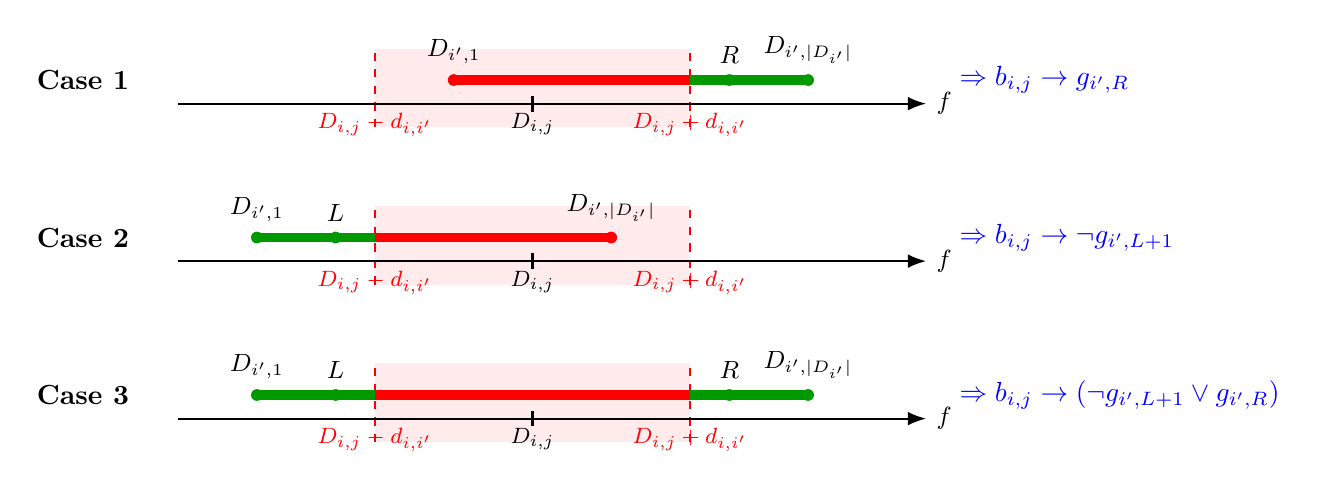
\begin{tikzpicture}[
    font=\small,
    axis/.style={-Latex, thick},
    forbidden/.style={fill=red!8},
    domain_invalid/.style={line width=3.5pt, red},
    domain_valid/.style={line width=3.5pt, green!60!black},
    domain_bound/.style={circle, fill, inner sep=1.5pt}
]

% Macros for repeated elements
\def\xCenter{4.5}
\def\d{2}
\def\fMin{\xCenter-\d} % 2.5
\def\fMax{\xCenter+\d} % 6.5

\newcommand{\drawBase}[2]{
    % Vùng cấm màu đỏ
    \fill[forbidden] (\fMin, #1-0.3) rectangle (\fMax, #1+0.7);
    \draw[red, dashed, thick] (\fMin, #1-0.3) -- (\fMin, #1+0.7);
    \draw[red, dashed, thick] (\fMax, #1-0.3) -- (\fMax, #1+0.7);

    % Trục f vẽ sau để nổi lên trên
    \draw[axis] (0, #1) -- (9.5, #1) node[right] {$f$};

    % Đánh dấu tâm D_{i,j} và giới hạn
    \draw[thick] (\xCenter, #1-0.1) -- (\xCenter, #1+0.1);
    \node[below, font=\footnotesize] at (\xCenter, #1) {$D_{i,j}$};
    \node[red, below, font=\footnotesize] at (\fMin, #1) {$D_{i,j}-d_{i,i'}$};
    \node[red, below, font=\footnotesize] at (\fMax, #1) {$D_{i,j}+d_{i,i'}$};

    % Tên Case
    \node[left, font=\bfseries] at (-0.5, #1+0.3) {#2};
}

% ==========================================
% Case 1: D_{i'} nằm trọn trong vùng cấm (eq:forbid_1)
% \drawBase{6}{Case 1}
% \draw[domain_invalid] (3, 6.3) -- (6, 6.3);
% \node[domain_bound, red, label=above:{$D_{i',1}$}] at (3, 6.3) {};
% \node[domain_bound, red, label=above:{$D_{i',|D_{i'}|}$}] at (6, 6.3) {};
% \node[right, font=\bfseries, text=blue] at (9.8, 6.3) {$\Rightarrow \neg b_{i,j}$};

% ==========================================
% Case 2: D_{i'} giao bên phải vùng cấm (eq:forbid_2)
\drawBase{4}{Case 1}
\draw[domain_invalid] (3.5, 4.3) -- (\fMax, 4.3);
\draw[domain_valid] (\fMax, 4.3) -- (8, 4.3);
\node[domain_bound, red, label=above:{$D_{i',1}$}] at (3.5, 4.3) {};
\node[domain_bound, green!60!black, label=above:{$D_{i',|D_{i'}|}$}] at (8, 4.3) {};
\node[domain_bound, green!60!black, label=above:{$R$}] at (7, 4.3) {};
\node[right, font=\bfseries, text=blue] at (9.8, 4.3) {$\Rightarrow b_{i,j} \rightarrow g_{i',R}$};

% ==========================================
% Case 3: D_{i'} giao bên trái vùng cấm (eq:forbid_3)
\drawBase{2}{Case 2}
\draw[domain_valid] (1, 2.3) -- (\fMin, 2.3);
\draw[domain_invalid] (\fMin, 2.3) -- (5.5, 2.3);
\node[domain_bound, green!60!black, label=above:{$D_{i',1}$}] at (1, 2.3) {};
\node[domain_bound, green!60!black, label=above:{$L$}] at (2, 2.3) {};
\node[domain_bound, red, label=above:{$D_{i',|D_{i'}|}$}] at (5.5, 2.3) {};
\node[right, font=\bfseries, text=blue] at (9.8, 2.3) {$\Rightarrow b_{i,j} \rightarrow \neg g_{i',L+1}$};

% ==========================================
% Case 4: D_{i'} trùm qua cả 2 bên vùng cấm (eq:forbid_4)
\drawBase{0}{Case 3}
\draw[domain_valid] (1, 0.3) -- (\fMin, 0.3);
\draw[domain_invalid] (\fMin, 0.3) -- (\fMax, 0.3);
\draw[domain_valid] (\fMax, 0.3) -- (8, 0.3);
\node[domain_bound, green!60!black, label=above:{$D_{i',1}$}] at (1, 0.3) {};
\node[domain_bound, green!60!black, label=above:{$L$}] at (2, 0.3) {};
\node[domain_bound, green!60!black, label=above:{$R$}] at (7, 0.3) {};
\node[domain_bound, green!60!black, label=above:{$D_{i',|D_{i'}|}$}] at (8, 0.3) {};
\node[right, font=\bfseries, text=blue] at (9.8, 0.3) {$\Rightarrow b_{i,j} \rightarrow (\neg g_{i',L+1} \lor g_{i',R})$};

\end{tikzpicture}
\caption{Visualization of the 4 domain pruning scenarios based on Order Encoding. The forbidden frequency interval $[D_{i,j} - d_{i,i'}, D_{i,j} + d_{i,i'}]$ caused by assigning $b_{i,j} = \text{True}$ is highlighted in red. The valid sub-domains for adjacent vertex $i'$ are marked in green, enforced by boundary variables $g_{i',R}$ and $\neg g_{i',L+1}$.}
\label{fig:domain_pruning_cases}
\end{figure*}

To elucidate the underlying mechanism of the aforementioned formulations, Fig. \ref{fig:domain_pruning_cases} visually illustrates the three interaction scenarios between the forbidden interval (red) and the valid frequency domain $D_{i'}$ (green) of the adjacent vertex $i'$. Instead of generating an overwhelming number of conflict clauses $\neg b_{i',k}$ for every single candidate frequency that falls into the forbidden zone (as required by the Direct SAT Encoding method), the proposed model efficiently bypasses this combinatorial explosion by establishing logical boundary points $L$ and $R$.

Specifically, in Case 1 (Equation \eqref{eq:forbid_1}) and Case 2 \eqref{eq:forbid_2}, where the valid frequencies of $D_{i'}$ reside exclusively on one side (either right or left) of the forbidden zone, the model employs logical implications to force the adjacent vertex $i'$ to either jump over the forbidden interval ($g_{i',R}$) or retreat behind the safe boundary ($\neg g_{i',L+1}$). Finally, Case 3 \eqref{eq:forbid_3} represents the most complex scenario, wherein the domain $D_{i'}$ spans across both sides of the forbidden interval. Here, the clause $(\neg g_{i',L+1} \lor g_{i',R})$ introduces a sharp logical branching: vertex $i'$ is strictly compelled to select a frequency residing in either the left or the right safe band.d. 

By establishing these logical ``barriers'' via the order variables $g$, the proposed encoding empowers the SAT solver to fully exploit the Unit Propagation mechanism, exhaustively pruning the infeasible holes in $O(1)$ time complexity. Furthermore, it is worth noting that Equations \eqref{eq:forbid_1}--\eqref{eq:forbid_3} inherently guarantee the interference prevention requirement, thereby seamlessly replacing the cumbersome inequality constraints (Equation \eqref{eq:sat_ineq}) of the DSE model.


\subsection{Objective Function Optimization via Incremental SAT}
\label{subsec:incremental_sat}

Once the baseline search space is established, the objective of the MO-FAP is to minimize the total number of distinct frequencies utilized. To track the network's overall state, let $D = \bigcup_{i \in V} D_i$ be the global set of all available frequencies in the system, sorted in ascending order with a total size of $N = |D|$. Let $D_{m}$ denote the frequency value at the $m$-th position within this set ($1 \le m \le N$).

We initialize a set of Boolean state variables $A_{m} \in \{\text{True}, \text{False}\}$, where $A_{m} = \text{True}$ if and only if the frequency $D_{m}$ is actively utilized by at least one transmitter. The logical dependency between the local vertex assignments (variables $b_{i,j}$) and the global frequency states is defined through the implication clauses in Equation \eqref{eq:active_link}. Fig. \ref{fig:b_to_A_implication} illustrates an example of this linkage mechanism.

\begin{align}
    b_{i,j} \rightarrow A_{m}, \quad \forall i \in V, \forall j, m : D_{i,j} = D_{m} \label{eq:active_link}
\end{align}

\begin{figure*}[htbp]
\centering
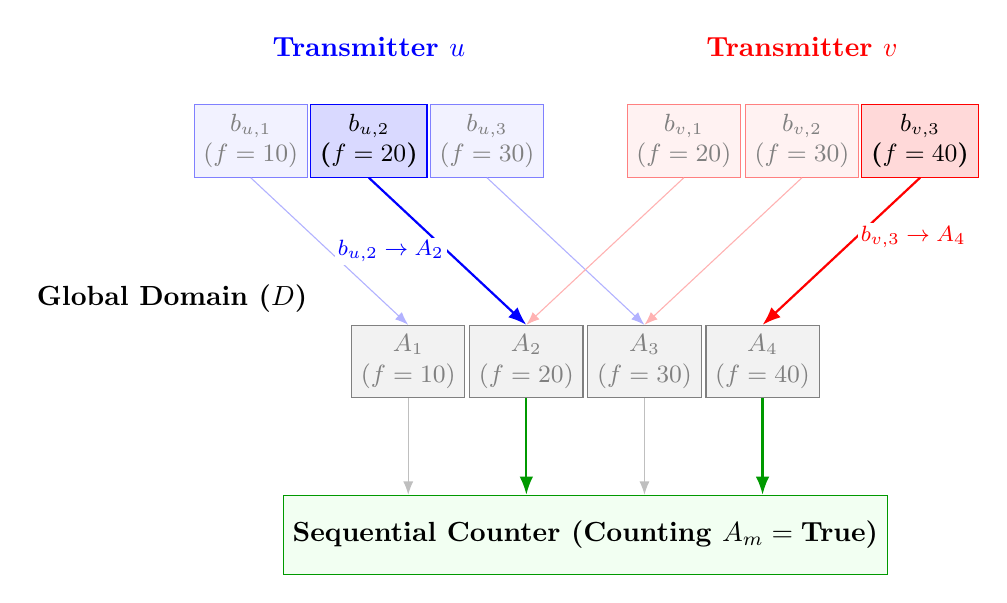
\begin{tikzpicture}[
    node distance = 1.5cm and 1cm,
    var_box/.style = {draw, rectangle, minimum width=1.2cm, minimum height=0.8cm, align=center, font=\small},
    % Style cho Trạm u (Màu Xanh)
    active_u/.style = {var_box, draw=blue, fill=blue!15, font=\small\bfseries},
    inactive_u/.style = {var_box, draw=blue!50, fill=blue!5, text=gray},
    arrow_u/.style = {-Latex, thick, blue},
    % Style cho Trạm v (Màu Đỏ)
    active_v/.style = {var_box, draw=red, fill=red!15, font=\small\bfseries},
    inactive_v/.style = {var_box, draw=red!50, fill=red!5, text=gray},
    arrow_v/.style = {-Latex, thick, red},
    % Style cho Biến Toàn cục A (Màu Xanh Lá)
    active_A/.style = {var_box, draw=green!60!black, fill=green!15, font=\small\bfseries},
    inactive_A/.style = {var_box, draw=gray, fill=gray!10, text=gray},
    arrow_A/.style = {-Latex, thick, green!60!black}
]

% --- Lớp trên: Trạm u và Trạm v (Local Domains) ---
% Trạm u
\node[text=blue] (u_label) at (-1.5, 2.2) {\textbf{Transmitter $u$}};
\node[inactive_u] (xu1) at (-3, 1) {$b_{u,1}$\\($f=10$)};
\node[active_u] (xu2) at (-1.5, 1) {$b_{u,2}$\\($f=20$)}; % Chọn f=20
\node[inactive_u] (xu3) at (0, 1) {$b_{u,3}$\\($f=30$)};

% Trạm v
\node[text=red] (v_label) at (4, 2.2) {\textbf{Transmitter $v$}};
\node[inactive_v] (xv1) at (2.5, 1) {$b_{v,1}$\\($f=20$)};
\node[inactive_v] (xv2) at (4, 1) {$b_{v,2}$\\($f=30$)};
\node[active_v] (xv3) at (5.5, 1) {$b_{v,3}$\\($f=40$)}; % Chọn f=40

% --- Lớp giữa: Global Frequency Pool (Các biến A) ---
\node (global_label) at (-4, -1) {\textbf{Global Domain ($D$)}};
\node[inactive_A] (A1) at (-1, -1.8) {$A_1$\\($f=10$)};
\node[inactive_A] (A2) at (0.5, -1.8) {$A_2$\\($f=20$)};
\node[inactive_A] (A3) at (2, -1.8) {$A_3$\\($f=30$)};
\node[inactive_A] (A4) at (3.5, -1.8) {$A_4$\\($f=40$)};

% --- Vẽ mũi tên lan truyền (Implications) ---
% Từ Trạm u (Màu Xanh Dương)
\draw[-Latex, draw=blue!30] (xu1.south) -- (A1.north);
\draw[arrow_u] (xu2.south) -- node[left, pos=0.5, font=\footnotesize, fill=white, inner sep=1pt] {$b_{u,2} \rightarrow A_2$} (A2.north);
\draw[-Latex, draw=blue!30] (xu3.south) -- (A3.north);

% Từ Trạm v (Màu Đỏ)
\draw[-Latex, draw=red!30] (xv1.south) -- (A2.north);
\draw[-Latex, draw=red!30] (xv2.south) -- (A3.north);
\draw[arrow_v] (xv3.south) -- node[right, pos=0.4, font=\footnotesize, fill=white, inner sep=1pt] {$b_{v,3} \rightarrow A_4$} (A4.north);

% --- Lớp dưới: Sequential Counter ---
\node[draw=green!60!black, rectangle, minimum width=6cm, minimum height=1cm, fill=green!5, font=\bfseries] (counter) at (1.25, -4) {Sequential Counter (Counting $A_{m} = \text{True}$)};

% Mũi tên từ A xuống Counter
\draw[-Latex, draw=gray!50] (A1.south) -- (A1.south |- counter.north);
\draw[arrow_A] (A2.south) -- (A2.south |- counter.north);
\draw[-Latex, draw=gray!50] (A3.south) -- (A3.south |- counter.north);
\draw[arrow_A] (A4.south) -- (A4.south |- counter.north);

\end{tikzpicture}
\caption{Illustration of the implication mechanism ($b_{i,j} \rightarrow A_{m}$) linking local frequency assignments to global active frequencies.}
\label{fig:b_to_A_implication}
\end{figure*}

The optimization of the objective function is executed via a linear search strategy. The algorithm begins by solving the baseline model to find an initial feasible solution, thereby establishing the initial Upper Bound ($UB$) for the number of utilized frequencies. In each subsequent iteration, the system is constrained to find a configuration using at most $k = UB - 1$ frequencies (an At-Most-$k$ constraint). If a valid configuration is found, the $UB$ is updated with the new value, and the loop continues until the solver returns \texttt{UNSAT}, which rigorously proves that the current $UB$ is the absolute global optimum.

Theoretically, these search iterations could be executed as independent solver calls. That is, for each new limit $k$, a fresh solver instance is initialized, the entire clause set is rebuilt from scratch, and the solving process restarts. However, this approach is highly inefficient because it forces the solver to restart, wiping out the entire search space state and the invaluable learned clauses accumulated during previous iterations. To optimize this process, we adopt the Incremental SAT technique \cite{martins2014incremental}, which allows the continuous reuse of the running solver across multiple iterations. 
% Within the Incremental SAT framework, there are two approaches to enforcing the active frequency limit.

To represent the objective function incrementally, modern SAT toolkits such as PySAT \cite{imms-sat18, itk-sat24} provide the (\texttt{ITotalizer}) encoding. 
In this method, the At-Most-$k$ clause set is constructed only once for the initial upper bound ($UB$). For subsequent iterations with smaller bounds ($k < UB$), the encoding utilizes a set of exposed control variables (assumptions) to restrict the number of active frequencies. 
However, the underlying binary tree structure of the Totalizer introduces a substantial number of auxiliary variables, and complex clause relationships. This topological complexity significantly increases the solving time.

Building upon the aforementioned paradigm of utilizing incremental control variables, we propose an optimized strategy that replaces the tree-based Totalizer with a Sequential Counter encoding \cite{Sinz2005}. The breakthrough of this method is that it perfectly inherits the $O(1)$ assumption-passing mechanism but drastically streamlines the logical topology. To thoroughly eliminate the structural overhead, the entire logical structure of the counter is generated and loaded into the solver only once with the initial maximum upper bound $K = UB$. Formally, a set of auxiliary variables $S_{i,c}$ ($1 \le i \le N, 1 \le c \le K$) is initialized, signifying that among the first $i$ frequencies, at least $c$ frequencies are in an active state. The logical clause block of the counter is rigidly established by Equations \eqref{eq:nsc_1}--\eqref{eq:nsc_7}:

\begin{align}
    & \bigwedge_{i=1}^{N} \left( A_i \rightarrow S_{i,1} \right) \label{eq:nsc_1} \\
    & \bigwedge_{i=2}^{N} \;\bigwedge_{c=1}^{\min(i-1,K)} \left( S_{i-1,c} \rightarrow S_{i,c} \right) \label{eq:nsc_2} \\
    & \bigwedge_{i=2}^{N} \;\bigwedge_{c=2}^{\min(i,K)} \left( A_i \land S_{i-1,c-1} \rightarrow S_{i,c} \right) \label{eq:nsc_3} \\
    & \bigwedge_{i=2}^{N} \;\bigwedge_{c=1}^{\min(i-1,K)} \left( \neg A_i \land \neg S_{i-1,c} \rightarrow \neg S_{i,c} \right) \label{eq:nsc_4} \\
    & \bigwedge_{i=1}^{K} \left( \neg A_i \rightarrow \neg S_{i,i} \right) \label{eq:nsc_5} \\
    & \bigwedge_{i=2}^{N} \;\bigwedge_{c=2}^{\min(i,K)} \left( \neg S_{i-1,c-1} \rightarrow \neg S_{i,c} \right) \label{eq:nsc_6} \\
    & \bigwedge_{i=K+1}^{N} \left( A_i \rightarrow \neg S_{i-1,K} \right) \label{eq:nsc_7}
\end{align}

Instead of adding new clauses to restrict the number of frequencies to $k < K$, we simply invoke the solver by passing a single \textit{Assumption} variable: $\neg S_{N, k+1}$ (assuming that it is impossible to have $\ge k+1$ active frequencies, which strictly enforces $\le k$). If the solver returns \texttt{SAT}, a new limit $UB' \le k$ is recorded. The system immediately retracts the old assumption in $O(1)$ time and invokes the next iteration with a tighter assumption, $\neg S_{N, UB'}$. 

This loop proceeds continuously until the SAT solver returns \texttt{UNSAT} or reaches the execution time limit (timeout). This \textit{Assumptions} passing strategy prevents the formula from expanding across iterations while allowing the solver to maintain the search tree intact and exploit 100\% of the knowledge from the learned clauses. Consequently, the proposed method completely eradicates the overhead of formula restructuring, drastically accelerating the convergence speed compared to the traditional restart approach.


\section{Experiments}
\label{sec:exp}
\subsection{Experimental Setup}

All experiments were conducted on a workstation equipped with an Intel Core i7-10850H processor and 16 GB of RAM, running the Ubuntu 24.04.3 LTS operating system. The SAT solving processes were executed using the CaDiCaL solver (version 1.9.5) via the Application Programming Interface (API) of the \texttt{PySAT} toolkit \cite{imms-sat18,itk-sat24}. To strictly control and accurately monitor the resource consumption of the algorithms, we integrated the \texttt{runlim} tool\footnote{\url{https://github.com/arminbiere/runlim/}}. For each solver instance, the system imposed strict computational boundaries: a maximum execution time (Time Limit) of 600 seconds and a maximum allocated memory (Memory Limit) of 14,000 MB. Any process exceeding these thresholds was forcefully terminated and recorded as either Timeout (TO) or Out of Memory (OOM), respectively.

The evaluations were performed on two standard benchmark datasets, CALMA and DUTtest, which have been widely verified in previous studies (archived in the FAP web database\textsuperscript{\ref{fn:fap_db}}). For the CALMA dataset, in addition to the instances originally designed for the Minimum Order Frequency Assignment Problem (MO-FAP), we expanded the evaluation space by reformulating the objective functions of all remaining CELAR and GRAPH instances into the MO-FAP format. This reformulation strategy is specifically intended to rigorously assess the solver's stability and pruning capabilities when dealing with inherently infeasible instances. Furthermore, to diversify the experimental dataset and provide a comprehensive evaluation, the DUTtest benchmark—also available from the aforementioned database—was incorporated into our experiments. Table \ref{tab:calma} summarizes the structural characteristics of the CALMA benchmark instances, where $|V|$ and $|E|$ denote the number of transceivers and distance constraints in the network, respectively.

% The evaluations were performed on two standard benchmark datasets, CALMA and DUTtest, which have been widely verified in previous studies (archived in the FAP web database\footnote{\url{https://fap.zib.de/}}). For the CALMA dataset, in addition to the instances originally designed for the Minimum Order Frequency Assignment Problem (MO-FAP), we expanded the evaluation space by reformulating the objective functions of all remaining instances into the MO-FAP format. Table \ref{tab:calma} summarizes the structural characteristics of the CALMA and DUTtest benchmark instances, where $|V|$ and $|E|$ denote the number of transceivers and distance constraints in the network, respectively.

\begin{table}[htbp]
\centering
\caption{Characteristics of CALMA and DUTtest benchmark instances}
\label{tab:calma}
\begin{tabular}{l l l r r}
\toprule
\textbf{Inst.} & \textbf{Original Name} & \textbf{Objective} & $|V|$ & $|E|$ \\
\midrule
C01 & CELAR 01 & Minimum Order        & 916 & 5548 \\
C02 & CELAR 02 & Minimum Order        & 200 & 1235 \\
C03 & CELAR 03 & Minimum Order        & 400 & 2760 \\
C04 & CELAR 04 & Minimum Order        & 680 & 3967 \\
C05 & CELAR 05 & Minimum Span         & 400 & 2598 \\
C06 & CELAR 06 & Minimum Interference & 200 & 1322 \\
C07 & CELAR 07 & Minimum Interference & 400 & 2865 \\
C08 & CELAR 08 & Minimum Interference & 916 & 5744 \\
C09 & CELAR 09 & Minimum Interference & 680 & 4103 \\
C10 & CELAR 10 & Minimum Interference & 680 & 4103 \\
C11 & CELAR 11 & Minimum Order        & 680 & 4103 \\
G01 & GRAPH 01 & Minimum Order        & 200 & 1134 \\
G02 & GRAPH 02 & Minimum Order        & 400 & 2245 \\
G03 & GRAPH 03 & Minimum Span         & 200 & 1134 \\
G04 & GRAPH 04 & Minimum Span         & 400 & 2244 \\
G05 & GRAPH 05 & Minimum Interference & 200 & 1134 \\
G06 & GRAPH 06 & Minimum Interference & 400 & 2170 \\
G07 & GRAPH 07 & Minimum Interference & 400 & 2170 \\
G08 & GRAPH 08 & Minimum Order        & 680 & 3757 \\
G09 & GRAPH 09 & Minimum Order        & 916 & 5246 \\
G10 & GRAPH 10 & Minimum Span         & 680 & 3907 \\
G11 & GRAPH 11 & Minimum Interference & 680 & 3757 \\
G12 & GRAPH 12 & Minimum Interference & 680 & 4017 \\
G13 & GRAPH 13 & Minimum Interference & 916 & 5273 \\
G14 & GRAPH 14 & Minimum Order        & 916 & 4638 \\
T2.1 & TUD200.1 & Minimum Order        & 200 & 1171 \\
T2.2 & TUD200.2 & Minimum Order        & 200 & 1143 \\
T2.3 & TUD200.3 & Minimum Order        & 200 & 1160 \\
T2.4 & TUD200.4 & Minimum Order/Span   & 200 & 1142 \\
T2.5 & TUD200.5 & Minimum Interference & 200 & 1125 \\
T9.1 & TUD916.1 & Minimum Order        & 916 & 5177 \\
T9.2 & TUD916.2 & Minimum Order        & 916 & 5173 \\
T9.3 & TUD916.3 & Minimum Order        & 916 & 5262 \\
T9.4 & TUD916.4 & Minimum Order/Span   & 916 & 5183 \\
T9.5 & TUD916.5 & Minimum Interference & 916 & 5213 \\
\bottomrule
\end{tabular}
\end{table}
To comprehensively and objectively evaluate the model's performance, a multi-dimensional benchmarking framework was established. First, the proposed encoding methodology was directly compared against the baseline encoding (Direct SAT Encoding) to highlight the efficacy of the domain pruning technique. Next, the overall strength of the proposed system was benchmarked against leading commercial optimization software, specifically the Mixed-Integer Programming (MIP) and Constraint Programming (CP) solvers provided by Gurobi (v12.0.3)\footnote{\url{https://www.gurobi.com}} and IBM ILOG CPLEX (v12.1.1)\footnote{\url{https://www.ibm.com/products/ilog-cplex-optimization-studio}}. Finally, to certify the quality and reliability of the obtained solutions, the experimental results were cross-referenced with the best-known optimal bounds from previous studies.

% To standardize the presentation of the results, the following notations are used to define the algorithmic components: \textbf{DSE} and \textbf{POSE} refer to the \textit{Direct SAT Encoding} and \textit{Proposed Order-based SAT Encoding} models, respectively. \textbf{INC} denotes the \textit{Naive Incremental Approach} strategy for the objective function, whereas \textbf{INCSC} represents the proposed objective function strategy utilizing the Sequential Counter (\textit{Proposed Incremental Approach}). The baseline solvers are denoted as \textbf{Gurobi}, \textbf{CPLEX-MIP}, and \textbf{CPLEX-CP}. A complete SAT method is denoted by combining the encoding method with the objective function strategy (e.g., \textbf{POSE+INCSC}).


To standardize the presentation of the experimental results and enhance readability, the notations used to define the algorithmic components and baseline solvers are summarized in Table \ref{tab:notations}. Regarding the objective function optimization, we evaluate two incremental strategies: \textbf{INCSC}, which is our proposed approach utilizing the Sequential Counter, and \textbf{INC}, which serves as a basic incremental approach utilizing the \texttt{ITotalizer} object provided by the \texttt{PySAT} library (where the formulas and control variables are internally managed by the library). A complete SAT-based method is denoted by combining the encoding model with the objective function strategy (e.g., \textbf{POSE+INCSC}).

\begin{table}[htbp]
\centering
\renewcommand{\arraystretch}{1.2} % Nới lỏng khoảng cách hàng theo chuẩn IEEE
\caption{Summary of Algorithmic Notations}
\label{tab:notations}
% Cột 1 căn trái (l), cột 2 ép xuống dòng với độ rộng 70% cột (p)
\begin{tabular}{l p{0.7\columnwidth}}
\hline
\textbf{Notation} & \textbf{Description} \\
\hline
\multicolumn{2}{c}{\textit{SAT Encoding Models}} \\
\hline
\textbf{DSE} & Direct SAT Encoding \\
\textbf{POSE} & Proposed Order-based SAT Encoding \\
\hline
\multicolumn{2}{c}{\textit{Objective Function Strategies}} \\
\hline
\textbf{INC} & Basic Incremental Approach (PySAT \texttt{ITotalizer}) \\
\textbf{INCSC} & Proposed Incremental Approach (Sequential Counter) \\
\hline
\multicolumn{2}{c}{\textit{Commercial Baseline Solvers}} \\
\hline
\textbf{Gurobi} & Mixed-Integer Programming solver by Gurobi \\
\textbf{CPLEX-MIP} & Mixed-Integer Programming solver by IBM ILOG \\
\textbf{CPLEX-CP} & Constraint Programming solver by IBM ILOG \\
\hline
\end{tabular}
\end{table}


\subsection{Evaluation of Domain Preprocessing}
\begin{table}[H]
\centering
\caption{Impact of Pre-processing on 35 benchmark instances}
\label{tab:preprocess_simple}
\begin{tabular}{l|c|c|c}
\toprule
\textbf{Method} & \textbf{Better Sol.} & \textbf{Faster Time} & \textbf{Total} \\
\midrule
POSE+INCSC & 0 & 28 & 28/35 \\
POSE+INC & 0 & 25 & 25/35 \\
DSE+INCSC & 0 & 22 & 22/35 \\
GUROBI & 0 & 21 & 21/35 \\
CPLEX-CP & 1 & 8 & 9/35 \\
CPLEX-MIP & 2 & 20 & 22/35 \\
\bottomrule
\end{tabular}
\\[0.1cm]
{\scriptsize Better Sol: Preprocessing < No preprocessing. Faster Time: Preprocessing < No preprocessing when the Sol. is equal.}
\end{table}
\begin{table}[H]
\centering
\caption{Pre-processing on 13 INF instances}
\label{tab:preprocess_inf}
% \tiny
\begin{tabular}{l|c|c|c}
\toprule
\textbf{Method} & \textbf{Better} & \textbf{Faster} & \textbf{Total} \\
\midrule
POSE+INCSC & 0 & 13 & 13/13 \\
POSE+INC & 0 & 12 & 12/13 \\
DSE+INCSC & 0 & 13 & 13/13 \\
GUROBI & 0 & 13 & 13/13 \\
CPLEX-CP & 0 & 5 & 5/13 \\
CPLEX-MIP & 0 & 13 & 13/13 \\
\bottomrule
\end{tabular}
\\[0.1cm]
{\scriptsize Better Sol: Preprocessing < No preprocessing. Faster Time: Preprocessing < No preprocessing when the Sol. is equal.}s
% {\scriptsize INF: scen06, scen07, scen08, scen09, scen10, graph05, graph06, graph07, graph11, graph12, graph13, TUD200.5, TUD916.5}
\end{table}

\begin{figure}[H]
    \centering
    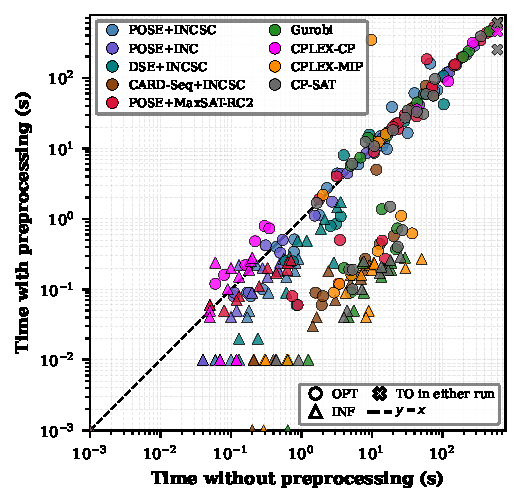
\includegraphics[width=\columnwidth]{image/iv_b_runtime_scatter_by_solver.png} 
    \caption{Impact of domain preprocessing on 35 benchmark instances. Points falling below the dashed $y=x$ line indicate a reduction in solving time when preprocessing is applied. The dense concentration of points in the lower-right region highlights significant speedup on computationally expensive instances.}
    \label{fig:preprocess_scatter}
\end{figure}


Problem reduction through preprocessing is highly effective for reducing the size of the initial problem formulation, as demonstrated in Tables \ref{tab:preprocess_simple} and \ref{tab:preprocess_inf}. 
The empirical data reveals that preprocessing acts as a powerful catalyst for both the SAT-based models and commercial solvers. 
Specifically, for the proposed \textbf{POSE+INCSC}, pruning invalid frequency domains successfully accelerates the search process in 80.00\% of the overall instances (28 out of 35). 
Moreover, it effectively rescues \textbf{CPLEX-MIP} and \textbf{CPLEX-CP} from severe time limitations in 2 and 1 highly constrained instances, respectively. 
The most profound impact, however, is observed in the 13 inherently infeasible (\texttt{INF}) instances, where the preprocessing technique accelerates the execution time in 100\% of the cases for \textbf{POSE+INCSC}, \textbf{DSE+INCSC}, \textbf{Gurobi}, and \textbf{CPLEX-MIP}. 
Many instances in the standard benchmark datasets were originally designed for other objectives (e.g., MS-FAP or MI-FAP) and have thus been reformulated to evaluate the MO-FAP. Because these original instances were already strictly constrained for their initial targets, the margin for further minimizing the number of assigned frequencies is extremely narrow. Nevertheless, the core purpose of utilizing these modified instances is to rigorously test the exact solvers' capability in search space pruning and proving infeasibility (\texttt{UNSAT}). Powered by the domain preprocessing technique combined with the SAT's unit propagation mechanism, the proposed model demonstrates an outstanding ability to certify the \texttt{UNSAT} status almost instantaneously.

The overall effectiveness is visually summarized in the scatter plot in Fig. \ref{fig:preprocess_scatter}. As observed, the vast majority of data points gravitate toward the region below the $y=x$ boundary, representing a consistent performance gain across a wide range of problem complexities.

\subsection{Evaluation of the Proposed Order-Based SAT Encoding}

\begin{table}[H]
\centering
\caption{Performance Comparison Between the Proposed Order-based SAT Encoding (POSE+INCSC) and Direct SAT Encoding (DSE+INCSC)}
\label{tab:pose_vs_dse}
\resizebox{\columnwidth}{!}{%
\small
\begin{tabular}{lcccccc}
\toprule
\textbf{Inst.} & \multicolumn{3}{c}{\textbf{POSE+INCSC}} & \multicolumn{3}{c}{\textbf{DSE+INCSC}} \\
\cmidrule(lr){2-4} \cmidrule(lr){5-7}
 & \textbf{Sol} & \textbf{Time} & \textbf{Status} & \textbf{Sol} & \textbf{Time} & \textbf{Status} \\
\midrule
C01 & 16 & \textbf{119.14} & \textbf{OPT} & 16 & 600.00 & TO \\
C02 & 14 & \textbf{9.78} & \textbf{OPT} & 14 & 600.00 & TO \\
C03 & 14 & \textbf{65.31} & \textbf{OPT} & 14 & 600.00 & TO \\
C04 & 46 & 0.10 & OPT & 46 & \textbf{0.07} & OPT \\
C05 & 40 & \textbf{0.40} & OPT & 40 & 0.79 & OPT \\
C06 & - & \textbf{0.22} & INF & - & 0.49 & INF \\
C07 & - & \textbf{0.19} & INF & - & 0.72 & INF \\
C08 & - & \textbf{0.27} & INF & - & 1.73 & INF \\
C09 & - & \textbf{0.01} & INF & - & 0.02 & INF \\
C10 & - & 0.01 & INF & - & 0.01 & INF \\
C11 & 22 & \textbf{16.49} & \textbf{OPT} & 22 & 600.00 & TO \\
G01 & 18 & \textbf{66.73} & \textbf{OPT} & 18 & 600.00 & TO \\
G02 & 14 & \textbf{14.96} & \textbf{OPT} & 14 & 600.00 & TO \\
G03 & 20 & \textbf{5.90} & OPT & 20 & 24.10 & OPT \\
G04 & 22 & \textbf{12.21} & OPT & 22 & 58.64 & OPT \\
G05 & - & \textbf{0.04} & INF & - & 0.09 & INF \\
G06 & - & \textbf{0.09} & INF & - & 0.49 & INF \\
G07 & - & 0.01 & INF & - & 0.01 & INF \\
G08 & 18 & \textbf{38.64} & \textbf{OPT} & 18 & 600.00 & TO \\
G09 & 18 & \textbf{159.46} & \textbf{OPT} & 18 & 600.00 & TO \\
G10 & 22 & \textbf{60.55} & \textbf{OPT} & 22 & 600.00 & TO \\
G11 & - & \textbf{0.15} & INF & - & 0.98 & INF \\
G12 & - & \textbf{0.01} & INF & - & 0.02 & INF \\
G13 & - & \textbf{0.24} & INF & - & 1.45 & INF \\
G14 & 8 & \textbf{8.64} & OPT & 8 & 106.29 & OPT \\
T2.1 & 12 & \textbf{2.74} & OPT & 12 & 42.02 & OPT \\
T2.2 & 46 & \textbf{0.08} & OPT & 46 & 0.26 & OPT \\
T2.3 & 14 & \textbf{1.13} & OPT & 14 & 8.00 & OPT \\
T2.4 & 20 & \textbf{0.09} & OPT & 20 & 0.25 & OPT \\
T2.5 & - & \textbf{0.05} & INF & - & 0.29 & INF \\
T9.1 & 18 & \textbf{10.87} & OPT & 18 & 58.76 & OPT \\
T9.2 & 48 & \textbf{0.34} & OPT & 48 & 0.86 & OPT \\
T9.3 & 24 & \textbf{4.40} & OPT & 24 & 15.68 & OPT \\
T9.4 & 26 & \textbf{0.51} & OPT & 26 & 1.08 & OPT \\
T9.5 & - & \textbf{0.18} & INF & - & 0.24 & INF \\
\midrule
\#OPT & 22 & & & 13 & & \\
\#INF & 13 & & & 13 & & \\
\#TO & 0 & & & 9 & & \\
\bottomrule
\end{tabular}%
}
\end{table}


This experiment evaluates the computational performance of the Proposed Order-based SAT Encoding (POSE) against the Direct SAT Encoding (DSE) baseline, with both utilizing domain preprocessing and the \textit{INCSC} strategy. 
Detailed results across 35 instances are presented in Table \ref{tab:pose_vs_dse}. The \textbf{Sol} column reports the minimum number of frequencies found, while \textbf{Time} records the execution time in seconds. The \textbf{Status} column indicates the solver's final state: \texttt{OPT} (optimal solution certified), \texttt{INF} (proven infeasible), or \texttt{TO} (600-second timeout). 
The final three rows tally the total occurrences of each state, explicitly highlighting how many instances each encoding successfully solved (\texttt{OPT} and \texttt{INF}) versus those it failed to resolve (\texttt{TO})

\begin{figure}[H]
\centering
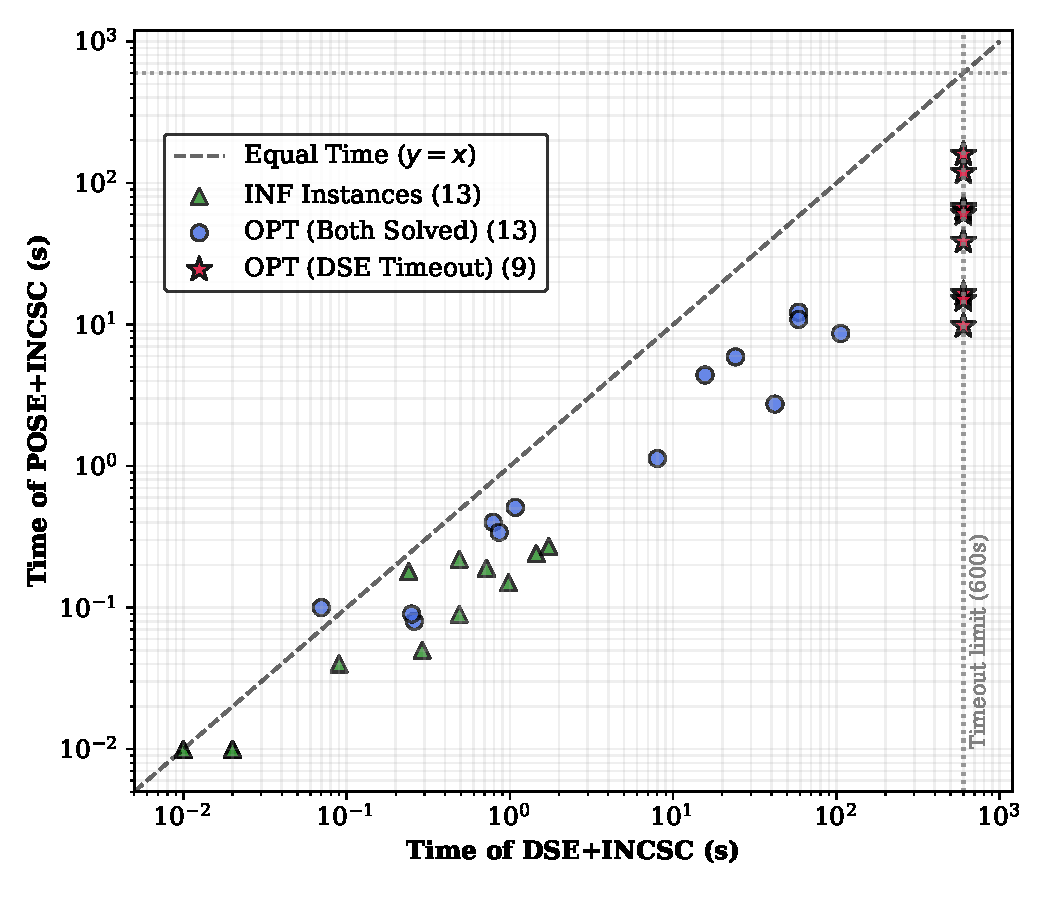
\includegraphics[width=0.95\columnwidth]{image/pose_vs_dse_scatter.pdf}
\caption{Log-log scatter plot comparing the execution times of DSE+INCSC and POSE+INCSC across 35 instances. The dashed line $y=x$ represents equal performance. Points located below this line indicate that POSE is faster.}
\label{fig:pose_vs_dse_scatter}
\end{figure}

To provide a more intuitive perspective on the performance disparity, Fig. \ref{fig:pose_vs_dse_scatter} visualizes the execution times of both encodings on a logarithmic scatter plot. The empirical data strongly validates the comprehensive superiority of POSE over the direct encoding approach in terms of both execution time and overall convergence capability. In particular, POSE successfully solves and mathematically certifies all 35 instances within the 600-second limit, achieving an absolute success rate of 100\%. As clearly depicted by the distribution of data points falling entirely below the $y=x$ reference line, the proposed POSE model consistently operates at a higher speed than the baseline.

In contrast, representing the distance constraints via discrete Boolean variables causes DSE to suffer from severe combinatorial explosions. This vulnerability is visually pronounced in Fig. \ref{fig:pose_vs_dse_scatter} by the distinct cluster of points pinned against the 600-second vertical boundary, highlighting the 9 highly constrained networks (such as the \texttt{C01}--\texttt{C03}, \texttt{C11}, and \texttt{G01}, \texttt{G02}, \texttt{G08}--\texttt{G10} series) where DSE becomes entirely intractable (\texttt{TO}). Even on instances where DSE manages to converge, POSE maintains a processing speed up to an order of magnitude faster, as highlighted by instance \texttt{T2.1} (2.74s vs. 42.02s) and \texttt{G14} (8.64s vs. 106.29s).

The structural power of the proposed encoding is further underscored by the inherently infeasible instances (\texttt{INF}). To conclusively certify an \texttt{INF} status (i.e., \texttt{UNSAT}), the exact solver is compelled to exhaustively traverse and prune the entire search space. The results demonstrate that POSE reaches the \texttt{UNSAT} conclusion strictly faster than, or equivalently to, DSE in 100\% of these test cases. This consistent disparity serves as robust evidence for the efficacy of the proposed order-based distance encoding, demonstrating that the established auxiliary variables $g$ effectively accelerate the unit propagation process without introducing computational overhead.

\begin{table}[H]
\centering
% \caption{Performance Comparison Between POSE+INCSC and POSE+INC}
\caption{Performance Comparison Between the Proposed Incremental Approach using Sequential Counter (POSE+INCSC) and the Basic Incremental Approach using ITotalizer (POSE+INC)}
\label{tab:pose_incsc_vs_inc}
\resizebox{\columnwidth}{!}{%
\small
\begin{tabular}{lcccccc}
\toprule
\textbf{Inst.} & \multicolumn{3}{c}{\textbf{POSE+INCSC}} & \multicolumn{3}{c}{\textbf{POSE+INC}} \\
\cmidrule(lr){2-4} \cmidrule(lr){5-7}
 & \textbf{Sol} & \textbf{Time} & \textbf{Status} & \textbf{Sol} & \textbf{Time} & \textbf{Status} \\
\midrule
C01 & 16 & \textbf{119.14} & OPT & 16 & 215.06 & OPT \\
C02 & 14 & \textbf{9.78} & OPT & 14 & 13.86 & OPT \\
C03 & 14 & \textbf{65.31} & OPT & 14 & 122.41 & OPT \\
C04 & 46 & 0.10 & OPT & 46 & \textbf{0.09} & OPT \\
C05 & 40 & \textbf{0.40} & OPT & 40 & 0.42 & OPT \\
C06 & - & 0.22 & INF & - & 0.22 & INF \\
C07 & - & \textbf{0.19} & INF & - & 0.20 & INF \\
C08 & - & 0.27 & INF & - & 0.27 & INF \\
C09 & - & 0.01 & INF & - & 0.01 & INF \\
C10 & - & 0.01 & INF & - & 0.01 & INF \\
C11 & 22 & 16.49 & OPT & 22 & \textbf{16.42} & OPT \\
G01 & 18 & \textbf{66.73} & OPT & 18 & 152.72 & OPT \\
G02 & 14 & \textbf{14.96} & OPT & 14 & 16.95 & OPT \\
G03 & 20 & 5.90 & OPT & 20 & \textbf{4.46} & OPT \\
G04 & 22 & 12.21 & OPT & 22 & \textbf{10.93} & OPT \\
G05 & - & 0.04 & INF & - & 0.04 & INF \\
G06 & - & 0.09 & INF & - & 0.09 & INF \\
G07 & - & 0.01 & INF & - & 0.01 & INF \\
G08 & 18 & \textbf{38.64} & OPT & 18 & 103.44 & OPT \\
G09 & 18 & \textbf{159.46} & OPT & 18 & 286.23 & OPT \\
G10 & 22 & 60.55 & OPT & 22 & \textbf{40.94} & OPT \\
G11 & - & 0.15 & INF & - & 0.15 & INF \\
G12 & - & 0.01 & INF & - & 0.01 & INF \\
G13 & - & 0.24 & INF & - & 0.24 & INF \\
G14 & 8 & 8.64 & OPT & 8 & \textbf{8.49} & OPT \\
T2.1 & 12 & 2.74 & OPT & 12 & \textbf{1.75} & OPT \\
T2.2 & 46 & 0.08 & OPT & 46 & 0.08 & OPT \\
T2.3 & 14 & 1.13 & OPT & 14 & \textbf{1.11} & OPT \\
T2.4 & 20 & 0.09 & OPT & 20 & 0.09 & OPT \\
T2.5 & - & 0.05 & INF & - & 0.05 & INF \\
T9.1 & 18 & \textbf{10.87} & OPT & 18 & 13.07 & OPT \\
T9.2 & 48 & 0.34 & OPT & 48 & \textbf{0.33} & OPT \\
T9.3 & 24 & 4.40 & OPT & 24 & \textbf{4.36} & OPT \\
T9.4 & 26 & 0.51 & OPT & 26 & \textbf{0.50} & OPT \\
T9.5 & - & 0.18 & INF & - & 0.18 & INF \\
\midrule
\#OPT & 22 & & & 22 & & \\
\#INF & 13 & & & 13 & & \\
\#TO  & 0 & & & 0 & & \\
\bottomrule
\end{tabular}%
}
\end{table}

\subsection{Evaluation of the Objective Function Optimization}

This experiment evaluates the computational performance of the proposed incremental optimization strategy (\textbf{INCSC}) against the baseline incremental approach (\textbf{INC}), with both implemented atop the \textbf{POSE} encoding architecture. The detailed results in Table \ref{tab:pose_incsc_vs_inc} demonstrate that while both methods strictly preserve global optimality and converge to identical objective values (\textbf{Sol}), \textbf{INCSC} exhibits a distinct superiority in execution speed, particularly on instances characterized by expansive search spaces and complex constraint structures.

\begin{figure*}[]
\centering
\includegraphics[width=\textwidth]{image/inc_vs_incsc_bar_log.png}
\caption{Relative execution time comparison between the proposed POSE+INCSC and baseline POSE+INC on selected computationally demanding instances. Percentages indicate the relative time saved (green, negative) or increased (red, positive) by utilizing the INCSC strategy.}
\label{fig:inc_vs_incsc_bar}
\end{figure*}

To visually quantify this acceleration, Fig. \ref{fig:inc_vs_incsc_bar} illustrates the relative execution time difference between the proposed \textbf{INCSC} strategy and the baseline \textbf{INC} approach for instances requiring more than 0.5 seconds to solve. A critical observation from the empirical data is the profound efficiency of \textbf{INCSC} on computationally demanding networks that require extensive search periods. Specifically, on highly constrained instances such as \texttt{C01}, \texttt{C03}, \texttt{G01}, \texttt{G08}, and \texttt{G09}, the Sequential Counter architecture dramatically accelerates convergence, reducing the total solving time by 44\% to over 62\% compared to \textbf{INC} (e.g., 119.14s vs. 215.06s for \texttt{C01}, and 38.64s vs. 103.44s for \texttt{G08}).

This significant acceleration stems directly from the underlying logical topology of the encodings. While both strategies efficiently utilize the assumption-passing mechanism to avoid rebuilding the formula across iterations, they differ drastically in their structural complexity. \textbf{INC} relies on the \texttt{ITotalizer}'s binary tree structure, which inherently introduces a massive number of auxiliary variables and convoluted clause relationships. This topological complexity artificially inflates the search space and heavily burdens the solver during unit propagation. Conversely, the Sequential Counter in \textbf{INCSC} maintains a flawlessly streamlined, linear logical structure. By passing a single assumption variable through this flat architecture, \textbf{INCSC} drastically minimizes structural overhead and provides a much faster, more direct path for the solver to prune unpromising branches.

Conversely, for simpler instances where the baseline reaches optimal solutions almost instantaneously (e.g., \texttt{C04}, \texttt{T2.1}, \texttt{T9.2}), \textbf{INCSC} occasionally records positive relative percentage increases. However, as depicted by the logarithmic y-axis in Fig. \ref{fig:inc_vs_incsc_bar}, the absolute execution times for these networks remain practically negligible (often under 5 seconds). The fraction of a second added is a marginal initialization trade-off that is overwhelmingly compensated by the substantial time savings achieved in large-scale scenarios (with \texttt{G10} being a rare topological exception). Furthermore, on inherently infeasible (\texttt{INF}) networks, the execution times of both methods are virtually identical, as the number of incremental bounding iterations is zero. 

Ultimately, these empirical findings unequivocally confirm that \textbf{INCSC} profoundly optimizes computational time by streamlining the logical search space, without compromising the mathematical rigor of the exact solutions.

% Hàm distance: Dùng chung cái của mình
% Hàm mục tiêu: nsc\_assumptions vs tot\_assumption

% Specifically, on highly demanding instances such as the \texttt{C01}--\texttt{C03} and \texttt{G01}--\texttt{G02} series, \textbf{INCSC} successfully reduces the total solving time by 30\% to over 50\% compared to \textbf{INC} (e.g., 119.14s vs. 215.06s for \texttt{C01}, and 66.73s vs. 152.72s for \texttt{G01}). This significant acceleration stems directly from the underlying logical topology of the encodings. While both strategies efficiently utilize the assumption-passing mechanism to avoid rebuilding the formula, they differ drastically in their structural complexity. \textbf{INC} relies on the \texttt{ITotalizer}'s binary tree structure, which inherently introduces a massive number of auxiliary variables and convoluted clause relationships. This topological complexity artificially inflates the search space and heavily burdens the solver during each incremental iteration. Conversely, the Sequential Counter in \textbf{INCSC} maintains a flawlessly streamlined, linear logical structure. By passing a single assumption variable through this flat architecture, \textbf{INCSC} drastically minimizes structural overhead and provides a much faster, more direct path for the solver's unit propagation.

% Conversely, on small-scale instances or inherently infeasible (\texttt{INF}) networks, the execution times of both methods are virtually identical, as the number of incremental bounding iterations is either negligible or zero. Ultimately, these empirical findings unequivocally confirm that \textbf{INCSC} profoundly optimizes computational time by streamlining the logical search space, without compromising the mathematical rigor of the exact solutions.



\subsection{Comparison with State-of-the-Art Exact Solvers}

\begin{table*}[htbp]
\centering
\caption{Comprehensive Comparison between Proposed POSE+INCSC and SOTA Solvers}
\label{tab:super_master}
\resizebox{\textwidth}{!}{%
\small
\begin{tabular}{l c ccc ccc ccc ccc} % Thêm 1 cột 'c' cho BKS
\toprule
\textbf{Instance} & \textbf{BKS\cite{Gomez2023MO}} & \multicolumn{3}{c}{\textbf{POSE+INCSC}} & \multicolumn{3}{c}{\textbf{Gurobi}} & \multicolumn{3}{c}{\textbf{CPLEX-CP}} & \multicolumn{3}{c}{\textbf{CPLEX-MIP}} \\
\cmidrule(lr){3-5} \cmidrule(lr){6-8} \cmidrule(lr){9-11} \cmidrule(lr){12-14} % Dịch cmidrule sang phải 1 cột
 & & \textbf{Solution} & \textbf{Time (s)} & \textbf{Status} & \textbf{Solution} & \textbf{Time (s)} & \textbf{Status} & \textbf{Solution} & \textbf{Time (s)} & \textbf{Status} & \textbf{Solution} & \textbf{Time (s)} & \textbf{Status} \\
\midrule
C01 & 16 & \textbf{16} & \textbf{119.14} & \textbf{OPT} & 20 & 600.00 & TO & \textbf{16} & 600.00 & TO & 24 & 600.00 & TO \\
C02 & 14 & \textbf{14} & 9.78 & \textbf{OPT} & \textbf{14} & \textbf{7.39} & \textbf{OPT} & \textbf{14} & 600.00 & TO & \textbf{14} & 600.00 & TO \\
C03 & 14 & \textbf{14} & \textbf{65.31} & \textbf{OPT} & 16 & 600.00 & TO & \textbf{14} & 600.00 & TO & 18 & 600.00 & TO \\
C04 & 46 & \textbf{46} & \textbf{0.10} & \textbf{OPT} & \textbf{46} & 0.16 & \textbf{OPT} & \textbf{46} & 0.22 & \textbf{OPT} & \textbf{46} & 0.12 & \textbf{OPT} \\
C05 & 40 & \textbf{40} & \textbf{0.40} & \textbf{OPT} & \textbf{40} & 1.37 & \textbf{OPT} & \textbf{40} & 0.73 & \textbf{OPT} & \textbf{40} & 1.10 & \textbf{OPT} \\
C06 & - & - & 0.22 & \textbf{INF} & - & 0.24 & \textbf{INF} & - & 0.24 & \textbf{INF} & - & 0.23 & \textbf{INF} \\
C07 & - & - & 0.19 & \textbf{INF} & - & 0.20 & \textbf{INF} & - & 0.20 & \textbf{INF} & - & 0.20 & \textbf{INF} \\
C08 & - & - & 0.27 & \textbf{INF} & - & 0.28 & \textbf{INF} & - & 0.28 & \textbf{INF} & - & 0.27 & \textbf{INF} \\
C09 & - & - & 0.01 & \textbf{INF} & - & 0.01 & \textbf{INF} & - & 0.01 & \textbf{INF} & - & 0.01 & \textbf{INF} \\
C10 & - & - & 0.01 & \textbf{INF} & - & 0.01 & \textbf{INF} & - & 0.01 & \textbf{INF} & - & 0.01 & \textbf{INF} \\
C11 & 22 & \textbf{22} & \textbf{16.49} & \textbf{OPT} & \textbf{22} & 198.57 & \textbf{OPT} & \textbf{22} & 600.00 & TO & 32 & 600.00 & TO \\
G01 & 18 & \textbf{18} & 66.73 & \textbf{OPT} & \textbf{18} & 5.68 & \textbf{OPT} & \textbf{18} & 600.00 & TO & \textbf{18} & \textbf{2.19} & \textbf{OPT} \\
G02 & 14 & \textbf{14} & \textbf{14.96} & \textbf{OPT} & \textbf{14} & 44.70 & \textbf{OPT} & \textbf{14} & 600.00 & TO & \textbf{14} & 15.97 & \textbf{OPT} \\
G03 & 20 & \textbf{20} & \textbf{5.90} & \textbf{OPT} & 22 & 600.00 & TO & \textbf{20} & 89.41 & \textbf{OPT} & 32 & 600.00 & TO \\
G04 & 22 & \textbf{22} & \textbf{12.21} & \textbf{OPT} & 44 & 600.00 & TO & \textbf{22} & 315.61 & \textbf{OPT} & - & 600.00 & TO \\
G05 & - & - & 0.04 & \textbf{INF} & - & 0.04 & \textbf{INF} & - & 0.04 & \textbf{INF} & - & 0.04 & \textbf{INF} \\
G06 & - & - & 0.09 & \textbf{INF} & - & 0.09 & \textbf{INF} & - & 0.10 & \textbf{INF} & - & 0.09 & \textbf{INF} \\
G07 & - & - & 0.01 & \textbf{INF} & - & 0.00 & \textbf{INF} & - & 0.01 & \textbf{INF} & - & 0.00 & \textbf{INF} \\
G08 & 18 & \textbf{18} & \textbf{38.64} & \textbf{OPT} & \textbf{18} & 240.57 & \textbf{OPT} & \textbf{18} & 600.00 & TO & 22 & 600.00 & TO \\
G09 & 18 & \textbf{18} & \textbf{159.46} & \textbf{OPT} & 26 & 600.00 & TO & \textbf{18} & 600.00 & TO & 28 & 600.00 & TO \\
G10 & 22 & \textbf{22} & \textbf{60.55} & \textbf{OPT} & - & 600.00 & TO & \textbf{22} & 600.00 & TO & - & 600.00 & TO \\
G11 & - & - & 0.15 & \textbf{INF} & - & 0.15 & \textbf{INF} & - & 0.15 & \textbf{INF} & - & 0.16 & \textbf{INF} \\
G12 & - & - & 0.01 & \textbf{INF} & - & 0.01 & \textbf{INF} & - & 0.01 & \textbf{INF} & - & 0.01 & \textbf{INF} \\
G13 & - & - & 0.24 & \textbf{INF} & - & 0.24 & \textbf{INF} & - & 0.25 & \textbf{INF} & - & 0.24 & \textbf{INF} \\
G14 & 8 & \textbf{8} & \textbf{8.64} & \textbf{OPT} & \textbf{8} & 456.71 & \textbf{OPT} & 10 & 600.00 & TO & 16 & 600.00 & TO \\
T2.1 & - & \textbf{12} & \textbf{2.74} & \textbf{OPT} & \textbf{12} & 14.22 & \textbf{OPT} & \textbf{12} & 600.00 & TO & \textbf{12} & 12.34 & \textbf{OPT} \\
T2.2 & - & \textbf{46} & \textbf{0.08} & \textbf{OPT} & \textbf{46} & 0.09 & \textbf{OPT} & \textbf{46} & 0.12 & \textbf{OPT} & \textbf{46} & 0.09 & \textbf{OPT} \\
T2.3 & - & \textbf{14} & \textbf{1.13} & \textbf{OPT} & \textbf{14} & 15.13 & \textbf{OPT} & \textbf{14} & 455.48 & \textbf{OPT} & \textbf{14} & 345.36 & \textbf{OPT} \\
T2.4 & - & \textbf{20} & \textbf{0.09} & \textbf{OPT} & \textbf{20} & 0.20 & \textbf{OPT} & \textbf{20} & 0.16 & \textbf{OPT} & \textbf{20} & 0.16 & \textbf{OPT} \\
T2.5 & - & - & 0.05 & \textbf{INF} & - & 0.05 & \textbf{INF} & - & 0.05 & \textbf{INF} & - & 0.05 & \textbf{INF} \\
T9.1 & - & \textbf{18} & \textbf{10.87} & \textbf{OPT} & - & 600.00 & TO & 22 & 600.00 & TO & 46 & 600.00 & TO \\
T9.2 & - & \textbf{48} & \textbf{0.34} & \textbf{OPT} & \textbf{48} & 0.37 & \textbf{OPT} & \textbf{48} & 0.48 & \textbf{OPT} & \textbf{48} & 0.35 & \textbf{OPT} \\
T9.3 & - & \textbf{24} & \textbf{4.40} & \textbf{OPT} & - & 600.00 & TO & \textbf{24} & 35.65 & \textbf{OPT} & 46 & 600.00 & TO \\
T9.4 & - & \textbf{26} & \textbf{0.51} & \textbf{OPT} & \textbf{26} & 0.73 & \textbf{OPT} & \textbf{26} & 0.79 & \textbf{OPT} & \textbf{26} & 0.62 & \textbf{OPT} \\
T9.5 & - & - & 0.18 & \textbf{INF} & - & 0.19 & \textbf{INF} & - & 0.19 & \textbf{INF} & - & 0.19 & \textbf{INF} \\
\midrule
\#OPT & & 22 & & & 14 & & & 10 & & & 10 & & \\
\#INF & & 13 & & & 13 & & & 13 & & & 13 & & \\
\#TO & & 0 & & & 8 & & & 12 & & & 12 & & \\
\bottomrule
\multicolumn{14}{l}{\scriptsize \textit{BKS: Best Known Solution \cite{Gomez2023MO}.}}
\end{tabular}%
}
\end{table*}


\begin{figure*}[]
\centering
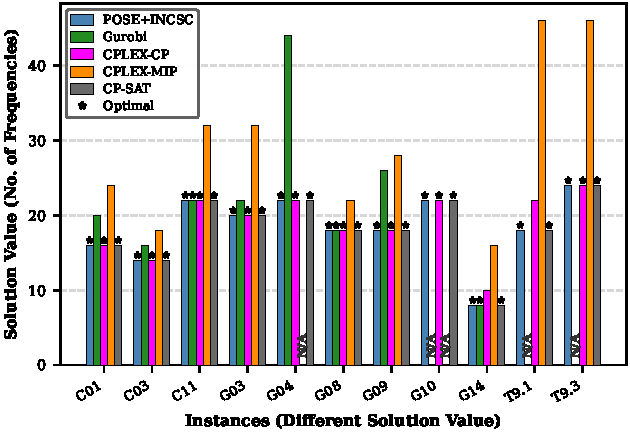
\includegraphics[width=2\columnwidth]{image/solution_quality_bar.png}
\caption{Solution quality comparison (objective value) on selected hard instances where baseline commercial solvers exceeded the 600s time limit. Lower values indicate a better solution (fewer frequencies used). Stars ($\star$) denote the optimal value achieved among the shown solvers for that instance. POSE+INCSC consistently achieves optimality in all cases, whereas commercial solvers (Gurobi, CPLEX-CP, CPLEX-MIP) frequently return sub-optimal bounds or fail to find any feasible solution (denoted as N/A) upon timeout.}
\label{fig:solution_quality}
\end{figure*}

\begin{figure}[]
\centering
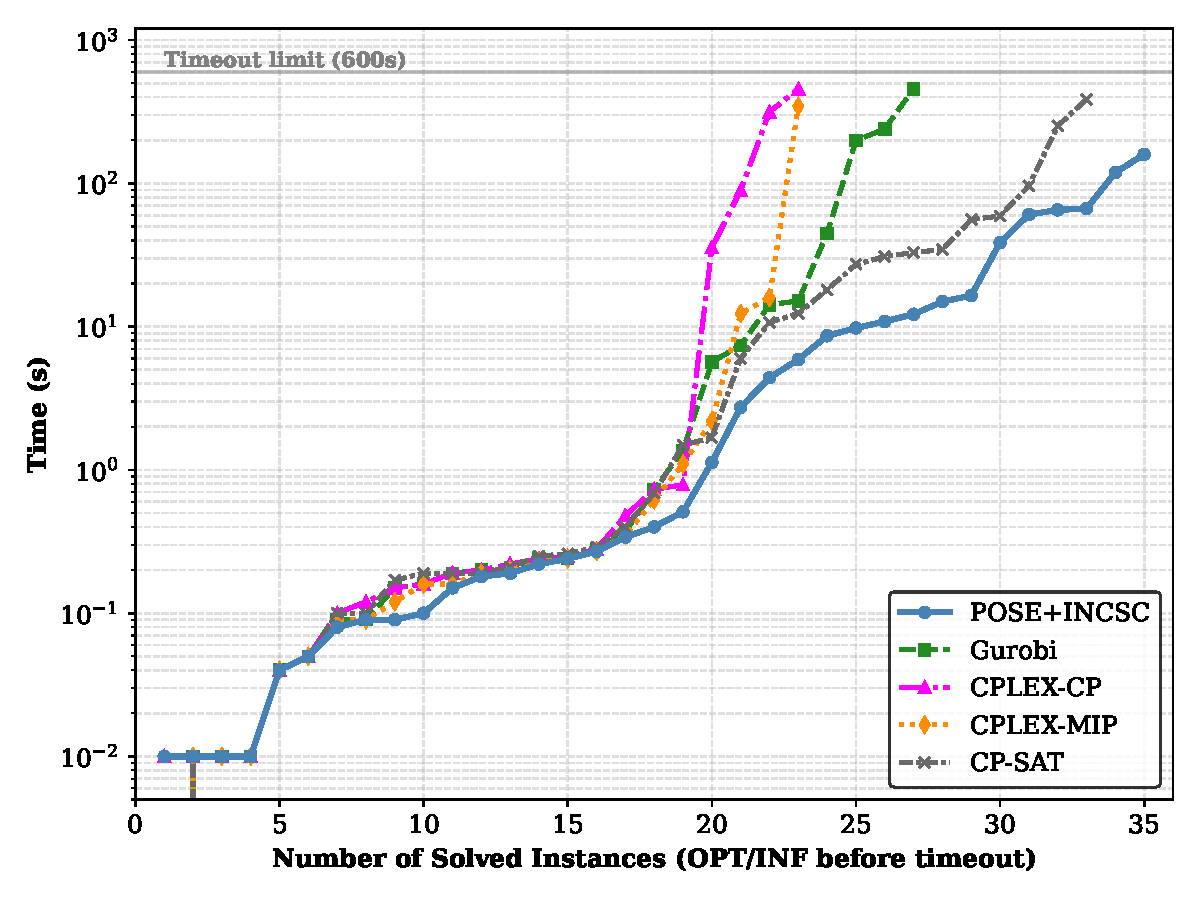
\includegraphics[width=\columnwidth ]{image/sota_cactus_plot.png}
\caption{Cactus plot comparing the overall performance of the proposed POSE+INCSC against Gurobi, CPLEX-CP, and CPLEX-MIP. The x-axis represents the number of successfully solved instances (OPT/INF before timeout), and the y-axis shows the required solving time in a logarithmic scale. A curve extending further to the right and staying lower indicates superior solver performance.}
\label{fig:sota_cactus}
\end{figure}

Finally, a comprehensive experiment was conducted to benchmark the proposed approach against the current state-of-the-art (SOTA) commercial solvers, specifically Gurobi, CPLEX-CP, and CPLEX-MIP. The detailed results in Table \ref{tab:super_master}, further visualized by the runtime distribution in Fig. \ref{fig:sota_cactus}, unequivocally demonstrate the multifaceted superiority of combining the POSE encoding with the INCSC strategy over traditional optimization technologies.

Regarding the overall convergence capability, the proposed method exhibits absolute dominance by successfully solving all 35 out of 35 instances, achieving a 100\% coverage rate. In stark contrast, the SOTA commercial solvers reveal significant limitations when navigating these densely constrained networks. As visually pronounced by the early termination of their respective curves in Fig. \ref{fig:sota_cactus}, CPLEX-CP and CPLEX-MIP manage to solve only 23 out of 35 instances (a 65.71\% success rate), suffering from severe combinatorial explosions and timing out (\texttt{TO}) on 12 test cases. Even Gurobi, which generally outperforms the CPLEX variants, fails to converge on 8 highly demanding instances (solving only 27 out of 35, or 77.14\%). The ability of the proposed system to consistently mathematically certify the global optimum (\texttt{OPT}) across all instances—particularly those where commercial solvers become completely intractable (e.g., \texttt{C01}--\texttt{C03}, \texttt{G08}--\texttt{G10})—highlights the profound stability and robustness of the POSE model combined with the INCSC strategy.

In terms of execution efficiency, as depicted by the trajectory of the proposed method remaining consistently low on the logarithmic y-axis of Fig. \ref{fig:sota_cactus}, the proposed system not only resolves a broader range of instances but also achieves drastically faster convergence speeds compared to the baselines. For instance, within the heavily constrained \texttt{TUD916} series (e.g., \texttt{T9.1} and \texttt{T9.3}), where the commercial solvers completely exhaust the 600-second time limit without yielding a conclusive result, the proposed method decisively finds and proves the optimal solution in merely 10.87s and 4.40s, respectively. Furthermore, for the inherently infeasible (\texttt{INF}) instances, the solving time of the proposed system is nearly instantaneous (often $\le 0.05$s). This exceptional performance indicates that the streamlined logical architecture of POSE profoundly empowers the SAT solver's Unit Propagation mechanism. By efficiently pruning unpromising branches and non-viable search spaces from the outset, the proposed framework minimizes computational overhead, thereby reaching the \texttt{OPT} or \texttt{INF} status with unprecedented speed and precision.


Furthermore, beyond execution speed, the gap in solution quality between the proposed method and the commercial baselines upon timeout is visually striking. Figure \ref{fig:solution_quality} focuses explicitly on challenging instances where the state-of-the-art solvers failed to converge within the 600-second limit. While CPLEX-CP occasionally managed to find the optimal bound (e.g., \texttt{C01}, \texttt{C03}, \texttt{TUD916.3}) before timing out—indicating a failure primarily in the proof phase rather than the search phase—both CPLEX-MIP and Gurobi suffered from severe performance degradation. For example, in \texttt{TUD916.1}, CPLEX-MIP returned a sub-optimal bound more than twice as large as the true optimal (46 vs. 18). More alarmingly, Gurobi completely failed to formulate even a single feasible solution (\texttt{N/A}) for highly constrained networks such as \texttt{G10}, \texttt{TUD916.1}, and \texttt{TUD916.3}, and returned heavily sub-optimal allocations for others like \texttt{G09}. This vividly demonstrates that not only does POSE+INCSC resolve all instances, but it consistently guarantees high-quality, mathematically optimal allocations where commercial alternatives often break down or provide practically unusable, high-cost solutions.

% Finally, a comprehensive experiment was conducted to benchmark the proposed approach against the current state-of-the-art (SOTA) commercial solvers, specifically Gurobi, CPLEX-CP, and CPLEX-MIP. The detailed results in Table \ref{tab:super_master} unequivocally demonstrate the multifaceted superiority of combining the POSE encoding with the INCSC strategy over traditional optimization technologies.

% Regarding the overall convergence capability, the proposed method exhibits absolute dominance by successfully solving all 35 out of 35 instances, achieving a 100\% coverage rate. In stark contrast, the SOTA commercial solvers reveal significant limitations when navigating these densely constrained networks. Specifically, CPLEX-CP and CPLEX-MIP manage to solve only 23 out of 35 instances (a 65.71\% success rate), suffering from severe combinatorial explosions and timing out (\texttt{TO}) on 12 test cases. Even Gurobi, which generally outperforms the CPLEX variants, fails to converge on 8 highly demanding instances (solving only 27 out of 35, or 77.14\%). The ability of the proposed system to consistently mathematically certify the global optimum (\texttt{OPT}) across all instances—particularly those where commercial solvers become completely intractable (e.g., \texttt{C01}--\texttt{C03}, \texttt{G08}--\texttt{G10})—highlights the profound stability and robustness of the POSE model combined with the INCSC strategy.

% In terms of execution efficiency, the proposed system not only resolves a broader range of instances but also achieves drastically faster convergence speeds compared to the baselines. For instance, within the heavily constrained \texttt{TUD916} series (e.g., \texttt{T9.1} and \texttt{T9.3}), where the commercial solvers completely exhaust the 600-second time limit without yielding a conclusive result, the proposed method decisively finds and proves the optimal solution in merely 10.87s and 4.40s, respectively. Furthermore, for the inherently infeasible (\texttt{INF}) instances, the execution time of the proposed system is nearly instantaneous (often $\le 0.05$s). This exceptional performance indicates that the streamlined logical architecture of POSE profoundly empowers the SAT solver's Unit Propagation mechanism. By efficiently pruning unpromising branches and non-viable search spaces from the outset, the proposed framework minimizes the computational overhead, thereby reaching the \texttt{OPT} or \texttt{INF} status with unprecedented speed and precision.

% \subsection{Nhận xét}
% % Đánh giá hiệu quả khi Pre-process. (Ngắn)
% Đánh giá hiệu quả Biểu diễn mới cho ràng buộc khoảng cách. So sánh với Naive SAT

% Đánh giá hiệu quả Biểu diễn hàm mục tiêu. So sánh dùng PB với dùng Sequential Counter. So với dùng at\_most\_k trực tiếp??

% Đánh giá tổng quan kết quả khi so với Baselines (Cplex, Gurobi).


\section{Conclusion}
\label{sec:conclusion}

In this paper, we proposed a novel exact approach based on Boolean Satisfiability (SAT) to solve and mathematically certify the global optimality of the Minimum Order Frequency Assignment Problem (MO-FAP). Transcending the inherent limitations of metaheuristic algorithms, which typically yield only approximate solutions, the proposed SAT framework provides a rigorous mathematical instrument to guarantee the absolute minimum frequency requirements for complex telecommunication networks.

The efficacy of the proposed system is anchored in two core technical contributions. First, the Proposed Order-based SAT Encoding (POSE) leverages auxiliary boundary variables to elegantly reformulate distance constraints. This structural innovation establishes logical safe zones, thereby empowering the solver to maximize unit propagation and aggressively prune unpromising search spaces. Second, the objective function optimization is driven by a novel Incremental Sequential Counter (INCSC) strategy coupled with an assumption-passing mechanism. This paradigm preserves the intact search tree across iterations, fully exploits accumulated learned clauses, and effectively eradicates the structural overhead and memory bottlenecks inherent in traditional binary tree encodings such as the \texttt{ITotalizer}.

Extensive computational experiments conducted on the standard CALMA and DUTtest benchmark datasets unequivocally validate the robustness of the proposed model. The \textbf{POSE+INCSC} framework achieved an absolute 100\% success rate (solving all 35 out of 35 instances) within the stringent time limit, demonstrating convergence speeds up to two orders of magnitude faster than leading state-of-the-art commercial solvers, including Gurobi and CPLEX. Crucially, the proposed SAT-based approach successfully circumvents the fundamental vulnerabilities of traditional Mixed-Integer Programming (MIP) models, particularly the numerical instability of Big-$M$ constants and weak linear relaxation bounds.

Looking ahead, this research trajectory can be naturally extended to address more intricate problem variants, such as the Minimum Span (MS-FAP) or Minimum Interference (MI-FAP) frequency assignment problems. Furthermore, integrating the proposed exact SAT formulations into hybrid frameworks, such as SAT-based Large Neighborhood Search (LNS), holds substantial promise for achieving unprecedented scalability in ultra-dense telecommunication networks tailored for the emerging 6G and IoT eras.

% \section{References Section}
\bibliographystyle{IEEEtran}
\bibliography{reference}


% \begin{figure}[htbp]
% \centering
% \begin{tikzpicture}
% \begin{semilogyaxis}[
%     width=\columnwidth, % Chiếm vừa vặn 1 cột của IEEE
%     height=6.5cm,
%     xlabel={Number of Solved Instances},
%     ylabel={Per-Instance Execution Time (s)},
%     xmin=0, xmax=35,
%     ymin=0.005, ymax=1000,
%     legend pos=north west,
%     legend style={font=\scriptsize, nodes={scale=0.85, transform shape}, fill=white, fill opacity=0.8, draw opacity=1, text opacity=1},
%     grid=both,
%     grid style={dashed, gray!30},
%     ytick={0.01, 0.1, 1, 10, 100, 600},
%     yticklabels={0.01, 0.1, 1, 10, 100, TO (600)},
%     extra y ticks={600},
%     extra y tick style={grid=major, grid style={red, dashed, thick}}
% ]

% % 1. Dữ liệu của Proposed (POSE+INCSC) - Giải được 35/35
% % (Lưu ý: Bạn lấy thời gian của 35 instances từ bảng của bạn, SẮP XẾP TĂNG DẦN rồi điền vào đây)
% \addplot[color=blue, mark=*, thick] coordinates {
%     (1, 0.01) (5, 0.01) (10, 0.10) (15, 0.29) 
%     (20, 0.69) (25, 3.34) (30, 14.63) (35, 106.02)
% };
% \addlegendentry{Proposed (POSE+INCSC)}

% % 2. Dữ liệu của Gurobi - Giải được 28/35
% \addplot[color=red, mark=square*, thick] coordinates {
%     (1, 0.01) (5, 0.02) (10, 0.22) (15, 2.44) 
%     (20, 5.53) (25, 17.43) (28, 248.56)
% };
% \addlegendentry{Gurobi}

% % 3. Dữ liệu của CPLEX-MIP - Giải được 20/35
% \addplot[color=orange, mark=triangle*, thick] coordinates {
%     (1, 0.01) (5, 0.22) (10, 9.67) 
%     (15, 45.71) (20, 531.92)
% };
% \addlegendentry{CPLEX-MIP}

% % 4. Dữ liệu của CPLEX-CP - Giải được 19/35
% \addplot[color=green!60!black, mark=diamond*, thick] coordinates {
%     (1, 0.01) (5, 0.22) (10, 7.28) 
%     (15, 31.32) (19, 496.46)
% };
% \addlegendentry{CPLEX-CP}

% \end{semilogyaxis}
% \end{tikzpicture}
% \caption{Cactus plot comparing the per-instance execution time and the number of solved instances among the proposed method and state-of-the-art commercial solvers. A strict time limit of 600 seconds is applied for each instance.}
% \label{fig:cactus_plot}
% \end{figure}

\end{document}


